%!TeX root = ../main.tex

\chapter{Performance Evaluation Results}\label{chapter:results}

This chapter presents and analyses the results of ten benchmarking experiments conducted across six EC2 instance types, directly answering the three research questions from Chapter~\ref{chapter:problem-statement}. The experiments span a network bandwidth progression from 10~Gbps to 200~Gbps, probing R2's throughput ceiling and latency behaviour under sustained high-concurrency workloads. Cost implications are then derived from the measured performance profile, closing the loop between the pricing analysis in Chapters~\ref{chapter:pricing}--\ref{chapter:migration} and the empirical evidence gathered here.

\section{Experimental Setup and Instance Configuration}\label{sec:experimental-setup}

To evaluate R2's throughput and latency characteristics across different network bandwidths and CPU configurations, six EC2 instance types were deployed in ten test runs, spanning from a 4-vCPU general-purpose instance to a 128-vCPU network-optimized platform. Table~\ref{tab:instance-config-summary} presents the complete test matrix, including instance specifications, configuration parameters, deployment regions, and test durations.

\begin{table}[H]
\centering
\caption{Complete instance configuration matrix for R2 performance evaluation}
\label{tab:instance-config-summary}
\footnotesize
\begin{tabular}{p{2.5cm}p{0.9cm}p{2.2cm}p{2.2cm}p{1.8cm}p{0.9cm}p{0.8cm}p{1cm}}
\hline
\textbf{Instance Type} & \textbf{vCPUs} & \textbf{Network \newline Bandwidth} & \textbf{Config (chunk/pipe)} & \textbf{Region (AWS)} & \textbf{Dur. (hrs)} & \textbf{Succ.} & \textbf{Max Conc.} \\
\hline
r5.xlarge       & 4   & 10 Gbps\textsuperscript{b} & 100 MB / p=3 & eu-north-1  & 0.24 & 100\% & C48 \\
r8gd.4xlarge    & 16  & 15 Gbps\textsuperscript{b} & 100 MB / p=3 & eu-central-1  & 0.24 & 100\% & C192 \\
r8gd.4xlarge-2  & 16  & 15 Gbps\textsuperscript{b} & 100 MB / p=3 & eu-central-1  & 1.19 & 100\% & C144 \\
r8gd.4xlarge-3  & 16  & 15 Gbps\textsuperscript{b} & 50 MB / p=6  & eu-central-1  & 1.19 & 100\% & C288 \\
c5n.9xlarge     & 36  & 50 Gbps          & 100 MB / p=3 & eu-north-1  & 0.19 & 100\% & C540 \\
c6in.16xlarge   & 64  & 100 Gbps         & 100 MB / p=3 & eu-north-1  & 0.25 & 100\% & C768 \\
hpc7g.16xlarge  & 64  & 200 Gbps (EFA)   & 100 MB / p=3 & eu-north-1  & 0.20 & 100\% & C576 \\
c6in.32xlarge   & 128 & 200 Gbps         & 100 MB / p=3 & eu-north-1  & 0.23 & 100\% & C1536 \\
c6in.32xlarge-2 & 128 & 200 Gbps         & 50 MB / p=6  & eu-north-1  & 0.21 & 100\% & C2304 \\
c6in.32xlarge-3 & 128 & 200 Gbps         & 50 MB / p=6  & eu-central-1 & 0.20 & 100\% & C2304 \\
\hline
\multicolumn{8}{l}{\textsuperscript{b} ``Up to X~Gbps'' instance (variable bandwidth, not guaranteed)} \\
\end{tabular}
\end{table}

The instance selection strategy followed a bandwidth progression from 10 Gbps to 200 Gbps, enabling systematic characterization of throughput scaling behavior. The r5.xlarge (4 vCPUs, 10 Gbps) and r8gd.4xlarge (16 vCPUs, 15 Gbps) represent baseline tiers for general-purpose workloads. The mid-tier instances --- c5n.9xlarge (36 vCPUs, 50 Gbps) and c6in.16xlarge (64 vCPUs, 100 Gbps) --- target high-performance network-bound applications. The high-tier configurations include the c6in.32xlarge (128 vCPUs, 200 Gbps) for maximum throughput, and the hpc7g.16xlarge (64 vCPUs, 200 Gbps EFA) to assess specialized interconnect performance for internet traffic.

\subsection{Workload Design and Configuration Rationale}

The workload consisted exclusively of byte-range GET requests targeting 50--100 MB segments from a single 9 GB object stored in R2. The 9 GB object size was selected as the maximum practical size within Cloudflare's free tier limit (10 GB total storage). Each request retrieved a random contiguous byte range, ensuring that no CloudFlare edge caching occurred between requests --- all traffic originated from R2's backend storage. This design choice isolates R2's core storage performance from CloudFlare's CDN layer, providing a worst-case baseline for direct storage access patterns.

The baseline configuration used 100 MB chunk sizes with HTTP pipeline depth of 3. The 100 MB chunk size was chosen to minimize the number of GET requests, thereby reducing per-request costs (\$0.36 per million requests). This reflects cost-conscious production scenarios where large-object batch transfers (backups, data pipelines, media processing) dominate egress patterns. The pipeline depth of 3 represents a conservative HTTP connection multiplexing factor that maintains sufficient in-flight data to saturate network links without overwhelming the client's connection pool.

For the c6in.32xlarge-2 configuration, chunk size was reduced to 50 MB and pipeline depth increased to 6. This parameter variation was introduced to observe system behavior under different request granularity, while maintaining approximately the same total in-flight data volume (100 MB $\times$ 3 $\approx$ 50 MB $\times$ 6). The c6in.32xlarge-3 deployment in Frankfurt (eu-central-1) rather than Stockholm (eu-north-1) enables comparison of network path quality to Cloudflare's global anycast infrastructure. All three r8gd.4xlarge experiments were conducted in the same region (eu-central-1, Frankfurt). The two r8gd.4xlarge long-run experiments are paired configurations with the same chunk$\times$pipeline product: r8gd.4xlarge-2 uses the baseline 100 MB / p=3 configuration (steady concurrency C=96), while r8gd.4xlarge-3 uses the 50 MB / p=6 configuration (steady concurrency C=192), matching the total in-flight data volume. Both runs were extended to approximately 1.2 hours to observe the bandwidth cliff under sustained load.

\subsection{Framework Configuration and Performance Metrics}

As described in Chapter~\ref{chapter:framework}, the benchmark framework uses a multi-process, asynchronous (coroutine-based) architecture with HTTP connection pooling. Each test progresses through the three-phase methodology defined in Section~\ref{sec:phases}: a warmup phase to stabilize TCP connections, followed by concurrency ramp steps where the number of workers per vCPU increments until throughput plateaus (Section~\ref{sec:plateau}), and finally a steady-state measurement phase at optimal concurrency. Total concurrency is computed as $C_{\text{total}} = N_{\text{cores}} \times W_{\text{per\_core}} \times D_{\text{pipeline}}$. For example, the c6in.32xlarge-2 configuration scaled from 768 (128 $\times$ 1 $\times$ 6) to 2,304 (128 $\times$ 3 $\times$ 6) concurrent HTTP connections.

The framework tracks two primary performance metrics:

\textbf{Throughput} is calculated as the total data volume transferred divided by the elapsed time, measured in gigabits per second (Gbps). For each test phase, throughput is computed as:
\[
\text{Throughput (Gbps)} = \frac{\text{Total Data (GB)} \times 8}{\text{Duration (seconds)}}
\]
This aggregate measure reflects the sustained network bandwidth utilization achieved by the client-server system as a whole.

\textbf{Latency} is measured at two levels: \textit{RTT (time-to-first-byte)} captures the delay from request initiation to receiving the first response byte, isolating queueing and processing overhead at R2's backend. \textit{Total latency} measures the complete request-response cycle including chunk download --- i.e., RTT plus data transfer time.

The framework's automatic retry logic (up to 3 attempts per request) masks transient network errors; reported success rates reflect post-retry outcomes.

\section{R2 Throughput Scalability Analysis}\label{sec:throughput-analysis}

Table~\ref{tab:throughput-summary} presents throughput results across all ten test runs. The r8gd.4xlarge long-run variants (-2, -3) share the same initial high-bandwidth peak as the base run but differ in average throughput due to a bandwidth cliff under extended sustained load; this behaviour is analysed in detail in Section~\ref{sec:latency-analysis}. The section proceeds by bandwidth tier to identify throughput ceilings and the factors limiting network utilization.

\begin{table}[H]
\centering
\caption{R2 throughput results across all test runs}
\label{tab:throughput-summary}
\small
\begin{tabular}{p{3cm}p{3cm}p{1.1cm}p{2.1cm}p{2.2cm}p{1.7cm}}
\hline
\textbf{Instance} & \textbf{NIC \newline Bandwidth} & \textbf{vCPUs} & \textbf{Peak (Gbps)} & \textbf{Avg (Gbps)} & \textbf{NIC Util.} \\
\hline
r5.xlarge          & 10 Gbps\textsuperscript{b}  & 4   & 6.7   & 6.1   & 67\% \\
r8gd.4xlarge       & 15 Gbps\textsuperscript{b}  & 16  & 14.3  & 12.9  & \textbf{95\%} \\
r8gd.4xlarge-2     & 15 Gbps\textsuperscript{b}  & 16  & 14.2  & 11.4\textsuperscript{c} & 95\%\textsuperscript{c} \\
r8gd.4xlarge-3     & 15 Gbps\textsuperscript{b}  & 16  & 14.3  & 11.7\textsuperscript{c} & 95\%\textsuperscript{c} \\
c5n.9xlarge        & 50 Gbps  & 36  & 41.0  & 39.5  & 82\% \\
c6in.16xlarge      & 100 Gbps & 64  & 78.4  & 73.5  & 78\% \\
hpc7g.16xlarge     & 200 Gbps (EFA) & 64 & 48.0 & 44.9 & 24\% \\
c6in.32xlarge      & 200 Gbps & 128 & 114.0 & 104.2 & 57\% \\
c6in.32xlarge-2    & 200 Gbps & 128 & \textbf{111.0} & 103.4 & 55\% \\
c6in.32xlarge-3    & 200 Gbps & 128 & 108.3 & 89.1  & 54\% \\
\hline
\multicolumn{6}{l}{\textsuperscript{b} ``Up to X~Gbps'' instance (variable bandwidth, not guaranteed)} \\
\multicolumn{6}{l}{\textsuperscript{c} Avg reduced by bandwidth cliff under sustained load; see Section~\ref{sec:latency-analysis}} \\
\end{tabular}
\end{table}

\subsection{Per-Core Processing Ceiling and Network Saturation}

CPU utilization measurements revealed sustained 90--99\% CPU load across all cores during peak throughput phases. This establishes a key characteristic of the Python-based client: the per-core achievable throughput is limited by per-request overhead (object allocation, metrics recording, asynchronous I/O bookkeeping), and decreases at higher core counts due to coordination overhead, memory bandwidth saturation, and Python runtime inefficiencies under high parallelism. On smaller instances (4 vCPUs), each core sustains roughly 1.5 Gbps; on 36--64 vCPU instances the ceiling is approximately 1.1--1.15 Gbps; on 128 vCPUs it drops to roughly 0.8 Gbps.

AWS EC2 imposes an additional constraint on traffic routed through the internet gateway, independent of the instance's NIC bandwidth. The AWS documentation states: \textit{``Bandwidth for multi-flow traffic is limited to 50\% of the available bandwidth for traffic that goes through an internet gateway \ldots\ for instances with 32 or more vCPUs, or 5~Gbps, whichever is larger. For instances with fewer than 32 vCPUs, bandwidth is limited to 5~Gbps.''}~\cite{aws-ec2-network-bandwidth}. The documentation further specifies that this cap applies independently to both inbound and outbound directions~\cite{aws-ec2-network-bandwidth}. Because the benchmark performs GET requests, the dominant traffic is \emph{inbound} to EC2 (large response bodies flowing in). Our workload generates many concurrent TCP connections, each a distinct 5-tuple flow, and therefore qualifies as multi-flow traffic through the internet gateway---meaning these documented limits nominally apply to our experimental setup.

The r8gd.4xlarge (16 vCPUs) is documented as an ``up to 15~Gbps'' instance, meaning 15~Gbps is the maximum non-guaranteed specification rather than a documented sustained level. The long-run experiments revealed the actual sustained level empirically: throughput held at 14.3~Gbps then dropped permanently to $\approx$7.1~Gbps at 28--37 minutes into steady state~\cite{aws-ec2-network-bandwidth}. The r5.xlarge similarly carries an ``up to'' specification (10~Gbps); its 14-minute test duration is insufficient to determine whether a comparable step-down would occur under longer load. Consequently, the reported throughput for both ``up to'' instances should be regarded as potentially reflecting elevated non-guaranteed conditions rather than confirmed sustained performance; the 32+ vCPU instances with fixed bandwidth specifications are not subject to this caveat.

For the 32+ vCPU instances, the theoretical IGW multi-flow caps are 25~Gbps (c5n.9xlarge, 50\% of 50~Gbps), 50~Gbps (c6in.16xlarge, 50\% of 100~Gbps), and 100~Gbps (c6in.32xlarge, 50\% of 200~Gbps). The measured averages of 39.5~Gbps and 73.5~Gbps for the 36- and 64-vCPU instances exceed their respective theoretical IGW caps by 58\% and 47\%. No enforcement of these documented limits was observed: the measured throughput exceeded the theoretical IGW caps despite the traffic nominally qualifying for the restriction. The reason is not determinable from client-side measurements alone; possible explanations include differences between documented nominal limits and actual AWS infrastructure enforcement in practice, or traffic-pattern-specific factors not visible to the client. The per-core CPU ceiling (36$\times$1.1$\approx$40~Gbps; 64$\times$1.15$\approx$74~Gbps) aligns closely with the measured values, making CPU the binding constraint for those instances. For the c6in.32xlarge, the CPU ceiling ($\approx$102~Gbps) and the IGW cap (100~Gbps) predict nearly identical throughput; the measured 104~Gbps cannot distinguish between them without further instrumentation. The practical implication for migration planning is clear regardless: any upload workload from an instance below 32 vCPUs faces a 5~Gbps documented IGW ceiling, and download-intensive workloads on 32+ vCPU instances should verify empirically whether throughput approaches the 50\% cap.


Whether an instance saturates its NIC therefore depends on whether the per-core throughput limit is reached before the NIC. Table~\ref{tab:throughput-per-vcpu} shows this for all configurations:

\begin{table}[H]
\centering
\caption{Per-vCPU throughput and network saturation across all instances}
\label{tab:throughput-per-vcpu}
\small
\begin{tabular}{p{2.8cm}p{1cm}p{1.8cm}p{1.8cm}p{1.8cm}p{3cm}}
\hline
\textbf{Instance} & \textbf{vCPUs} & \textbf{Avg (Gbps)} & \textbf{Gbps/vCPU needed} & \textbf{Gbps/vCPU achieved} & \textbf{Bottleneck} \\
\hline
r5.xlarge          & 4   & 6.1   & 2.50 & 1.53 & CPU \\
r8gd.4xlarge       & 16  & 12.9  & 0.94 & 0.81 & \textbf{NIC (95\%)} \\
c5n.9xlarge        & 36  & 39.5  & 1.39 & 1.10 & CPU \\
c6in.16xlarge      & 64  & 73.5  & 1.56 & 1.15 & CPU \\
hpc7g.16xlarge     & 64  & 44.9  & 3.13 & 0.70 & EFA (unsuitable) \\
c6in.32xlarge      & 128 & 104.2 & 1.56 & 0.81 & CPU \\
c6in.32xlarge-2    & 128 & 103.4 & 1.56 & 0.81 & CPU \\
c6in.32xlarge-3    & 128 & 89.1  & 1.56 & 0.70 & CPU + routing \\
\hline
\end{tabular}
\end{table}

On the r8gd.4xlarge, each core only needs to handle 0.94 Gbps (15 Gbps $\div$ 16 vCPUs), which falls within the per-core processing range --- so the NIC fills up before the CPUs do, achieving 95\% utilization. On the c6in.32xlarge (128 vCPUs), each core would need to handle 1.56 Gbps to saturate the 200 Gbps interface, exceeding what each core can deliver at this parallelism level --- so the CPUs max out first and the NIC reaches only 55--57\% utilization. The r5.xlarge (4 vCPUs) is CPU-limited at the aggregate level: each core delivers 1.53~Gbps, and 4$\times$1.53$\approx$6.1~Gbps matches the measured output exactly. The required 2.50~Gbps/core to saturate the 10~Gbps NIC exceeds the per-core limit, so the NIC is not reached. The measured 6.1~Gbps also exceeds the documented 5~Gbps multi-flow IGW cap for instances below 32~vCPUs, consistent with the ``up to 10~Gbps'' variable specification delivering above the sustained guaranteed level during this test window.

\subsection{Baseline Tier: 10--15 Gbps Instances}

The r5.xlarge instance achieved 6.7 Gbps peak throughput, representing 67\% of its nominal 10 Gbps capacity. Throughput plateaued between concurrency levels C24 and C48 (6.63--6.72 Gbps), while RTT escalated from 152 ms at C12 to 3,486 ms at C48. With 4 vCPUs, each core sustained 1.53 Gbps (6.1 Gbps $\div$ 4 vCPUs), consistent with the higher per-core efficiency at low parallelism. The ``up to 10~Gbps'' specification reflects variable non-guaranteed bandwidth; the EC2 multi-flow cap for instances below 32 vCPUs is 5~Gbps, and the measured 6.1~Gbps exceeds this cap. The 14-minute test duration was insufficient to determine whether throughput would have declined under longer sustained load~\cite{aws-ec2-network-bandwidth}.

The r8gd.4xlarge instance achieved 14.24 Gbps peak throughput, representing 95\% utilization of its 15 Gbps interface --- the highest network utilization of any configuration in this study. Figure~\ref{fig:r8gd-throughput-timeline} shows clean scaling from 10.5 Gbps at C48 to 14.2 Gbps at C96, then plateau at 14.24 Gbps (C144). This near-saturation demonstrates that no observable throttling was detected from R2 under tested conditions at the 15~Gbps scale; the client successfully saturated the interface.

\begin{figure}[H]
\centering
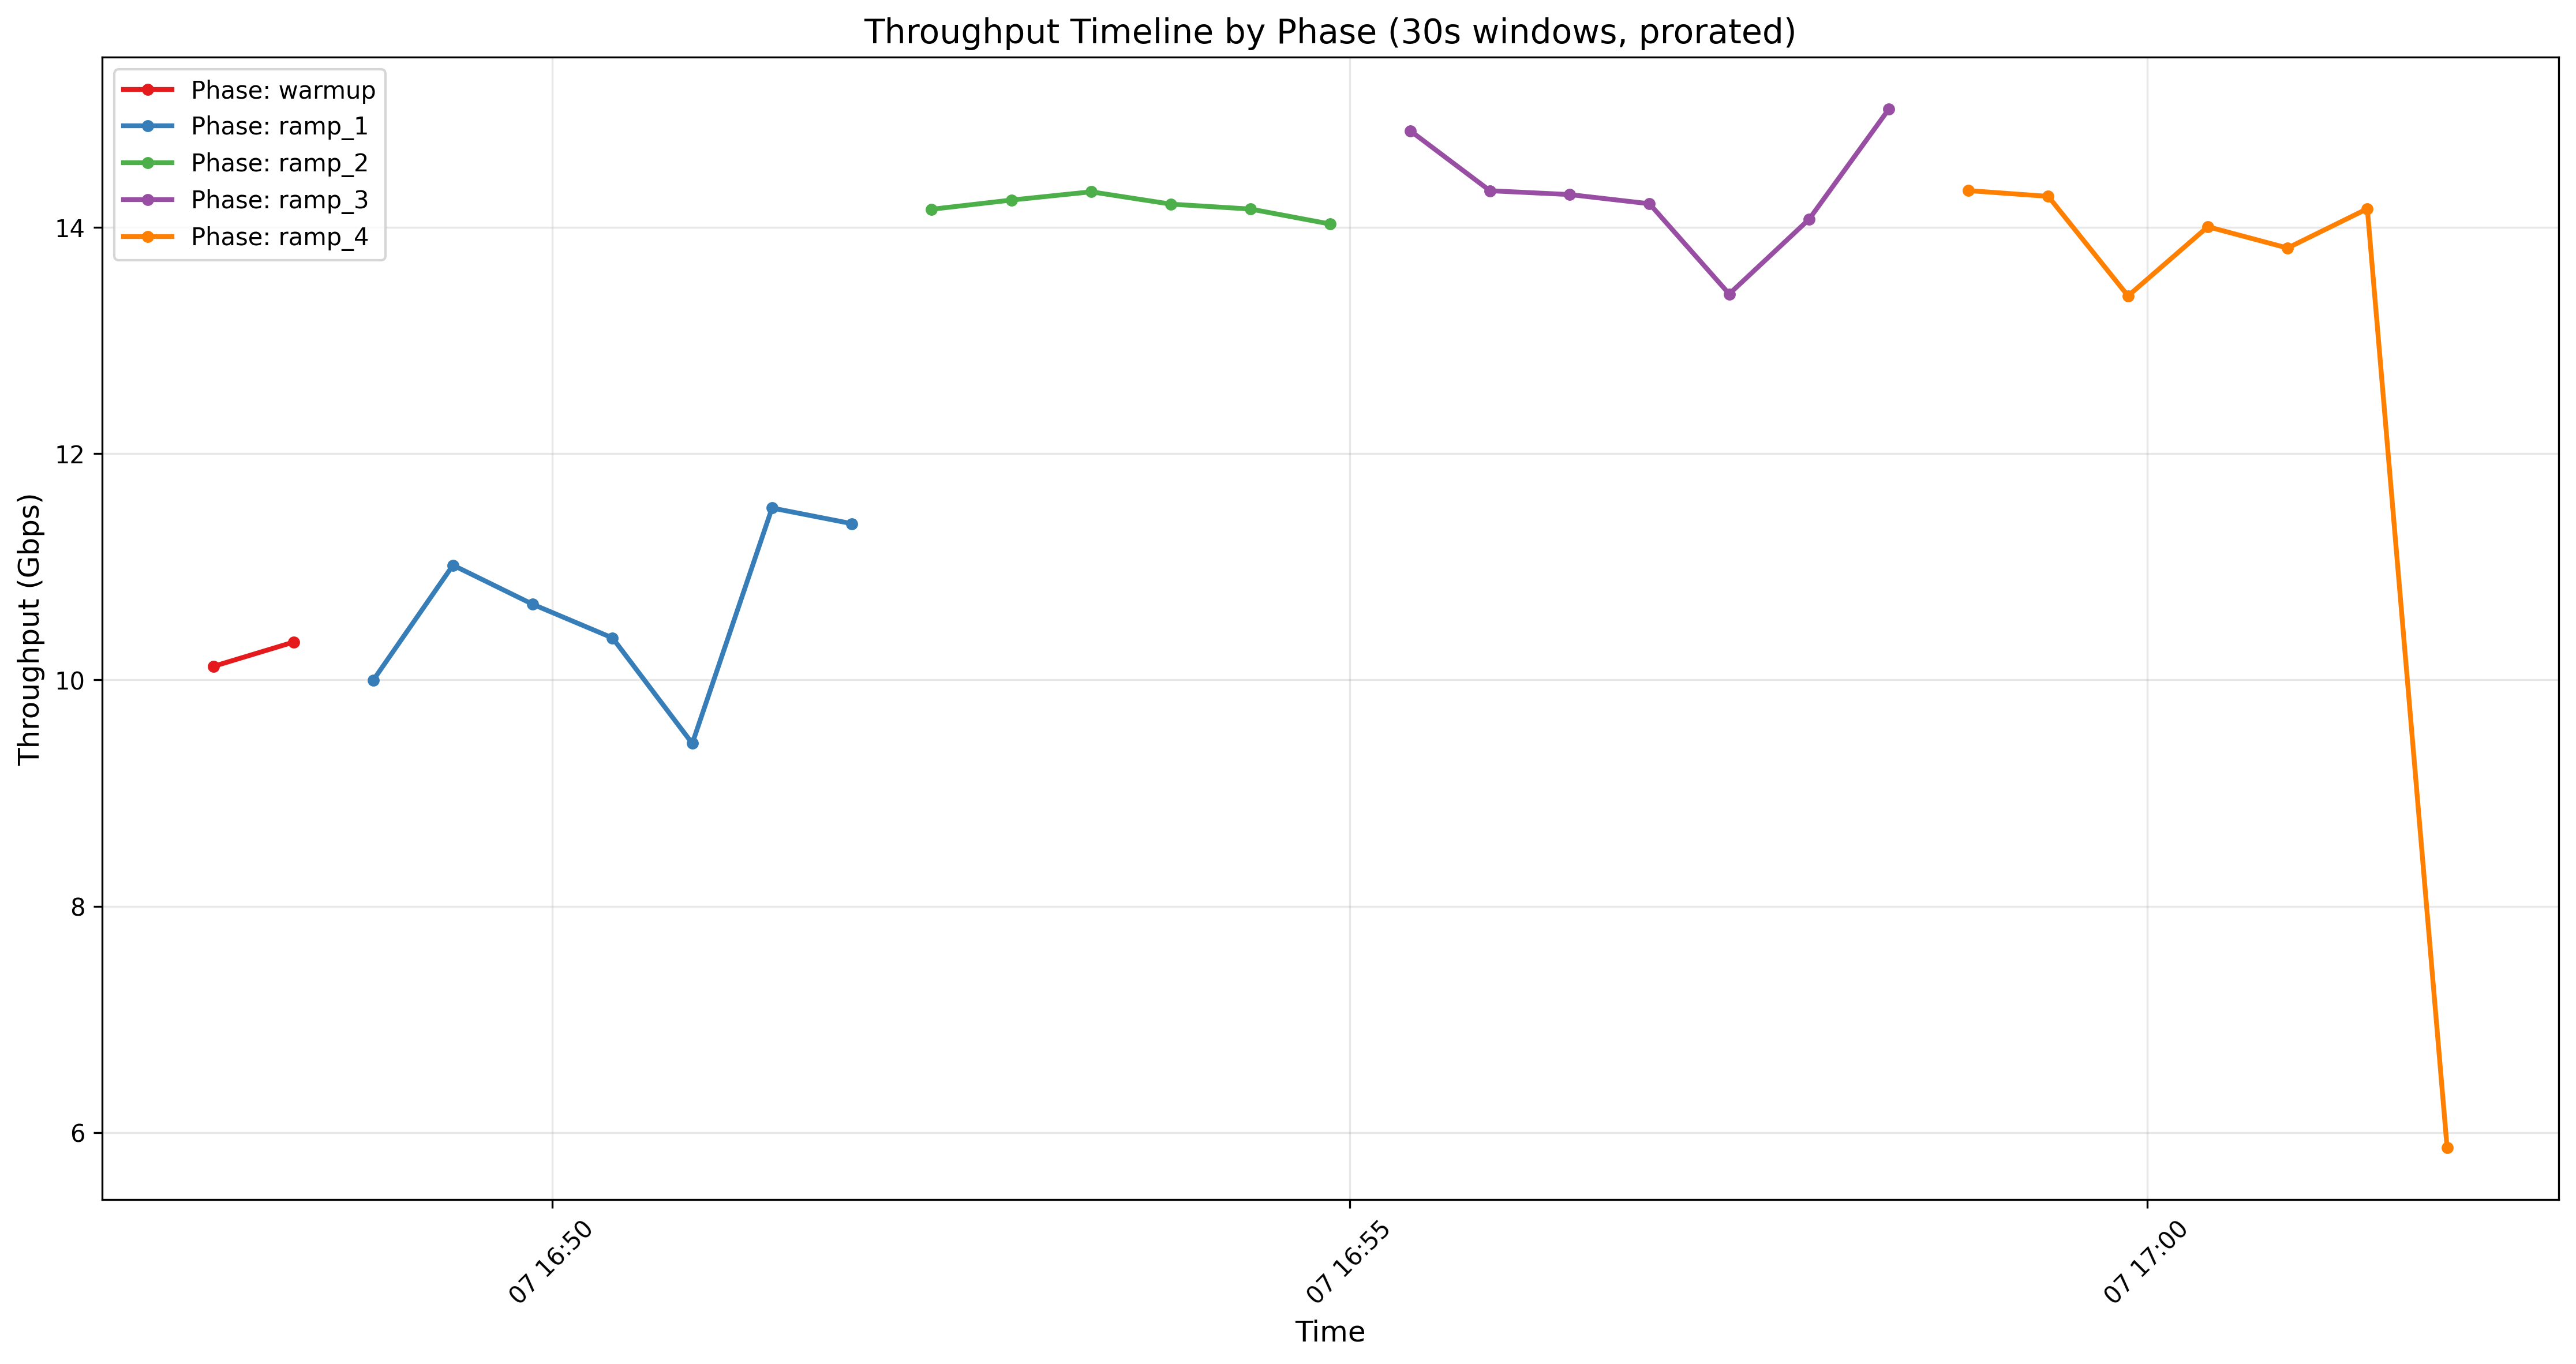
\includegraphics[width=\textwidth]{figures/r8gd-4xlarge-throughput_timeline.png}
\caption{R2 throughput timeline on r8gd.4xlarge (15 Gbps, 95\% utilization)}
\label{fig:r8gd-throughput-timeline}
\end{figure}

\subsection{Mid Tier: 50--100 Gbps Instances}

The c5n.9xlarge instance (36 vCPUs, 50 Gbps) achieved 41.0 Gbps peak and 39.5 Gbps average, representing 82\% utilization. Throughput peaked at C324 (40.9 Gbps) and declined slightly at higher concurrency (38.0 Gbps at C540). This establishes the first clear throughput ceiling at approximately 40 Gbps, consistent with the per-core processing limit: 36 vCPUs $\times$ 1.1 Gbps/core $\approx$ 40 Gbps theoretical maximum.

Doubling vCPU count from c5n.9xlarge's 36 cores to c6in.16xlarge's 64 cores (1.78×) yielded only 1.86× throughput improvement (39.5 $\to$ 73.5 Gbps), indicating diminishing returns as concurrency scales.

The c6in.16xlarge instance (64 vCPUs, 100 Gbps) achieved 78.4 Gbps peak and 73.5 Gbps average, representing 78\% utilization. Figure~\ref{fig:c6in16-throughput-vs-concurrency} shows an inverted-U pattern: throughput rose from 65.8 Gbps at C192 to a peak of 78.4 Gbps at C384, then declined slightly to 72--75 Gbps at C576--C768 as additional concurrency raised queueing pressure without proportional throughput gain.

\begin{figure}[H]
\centering
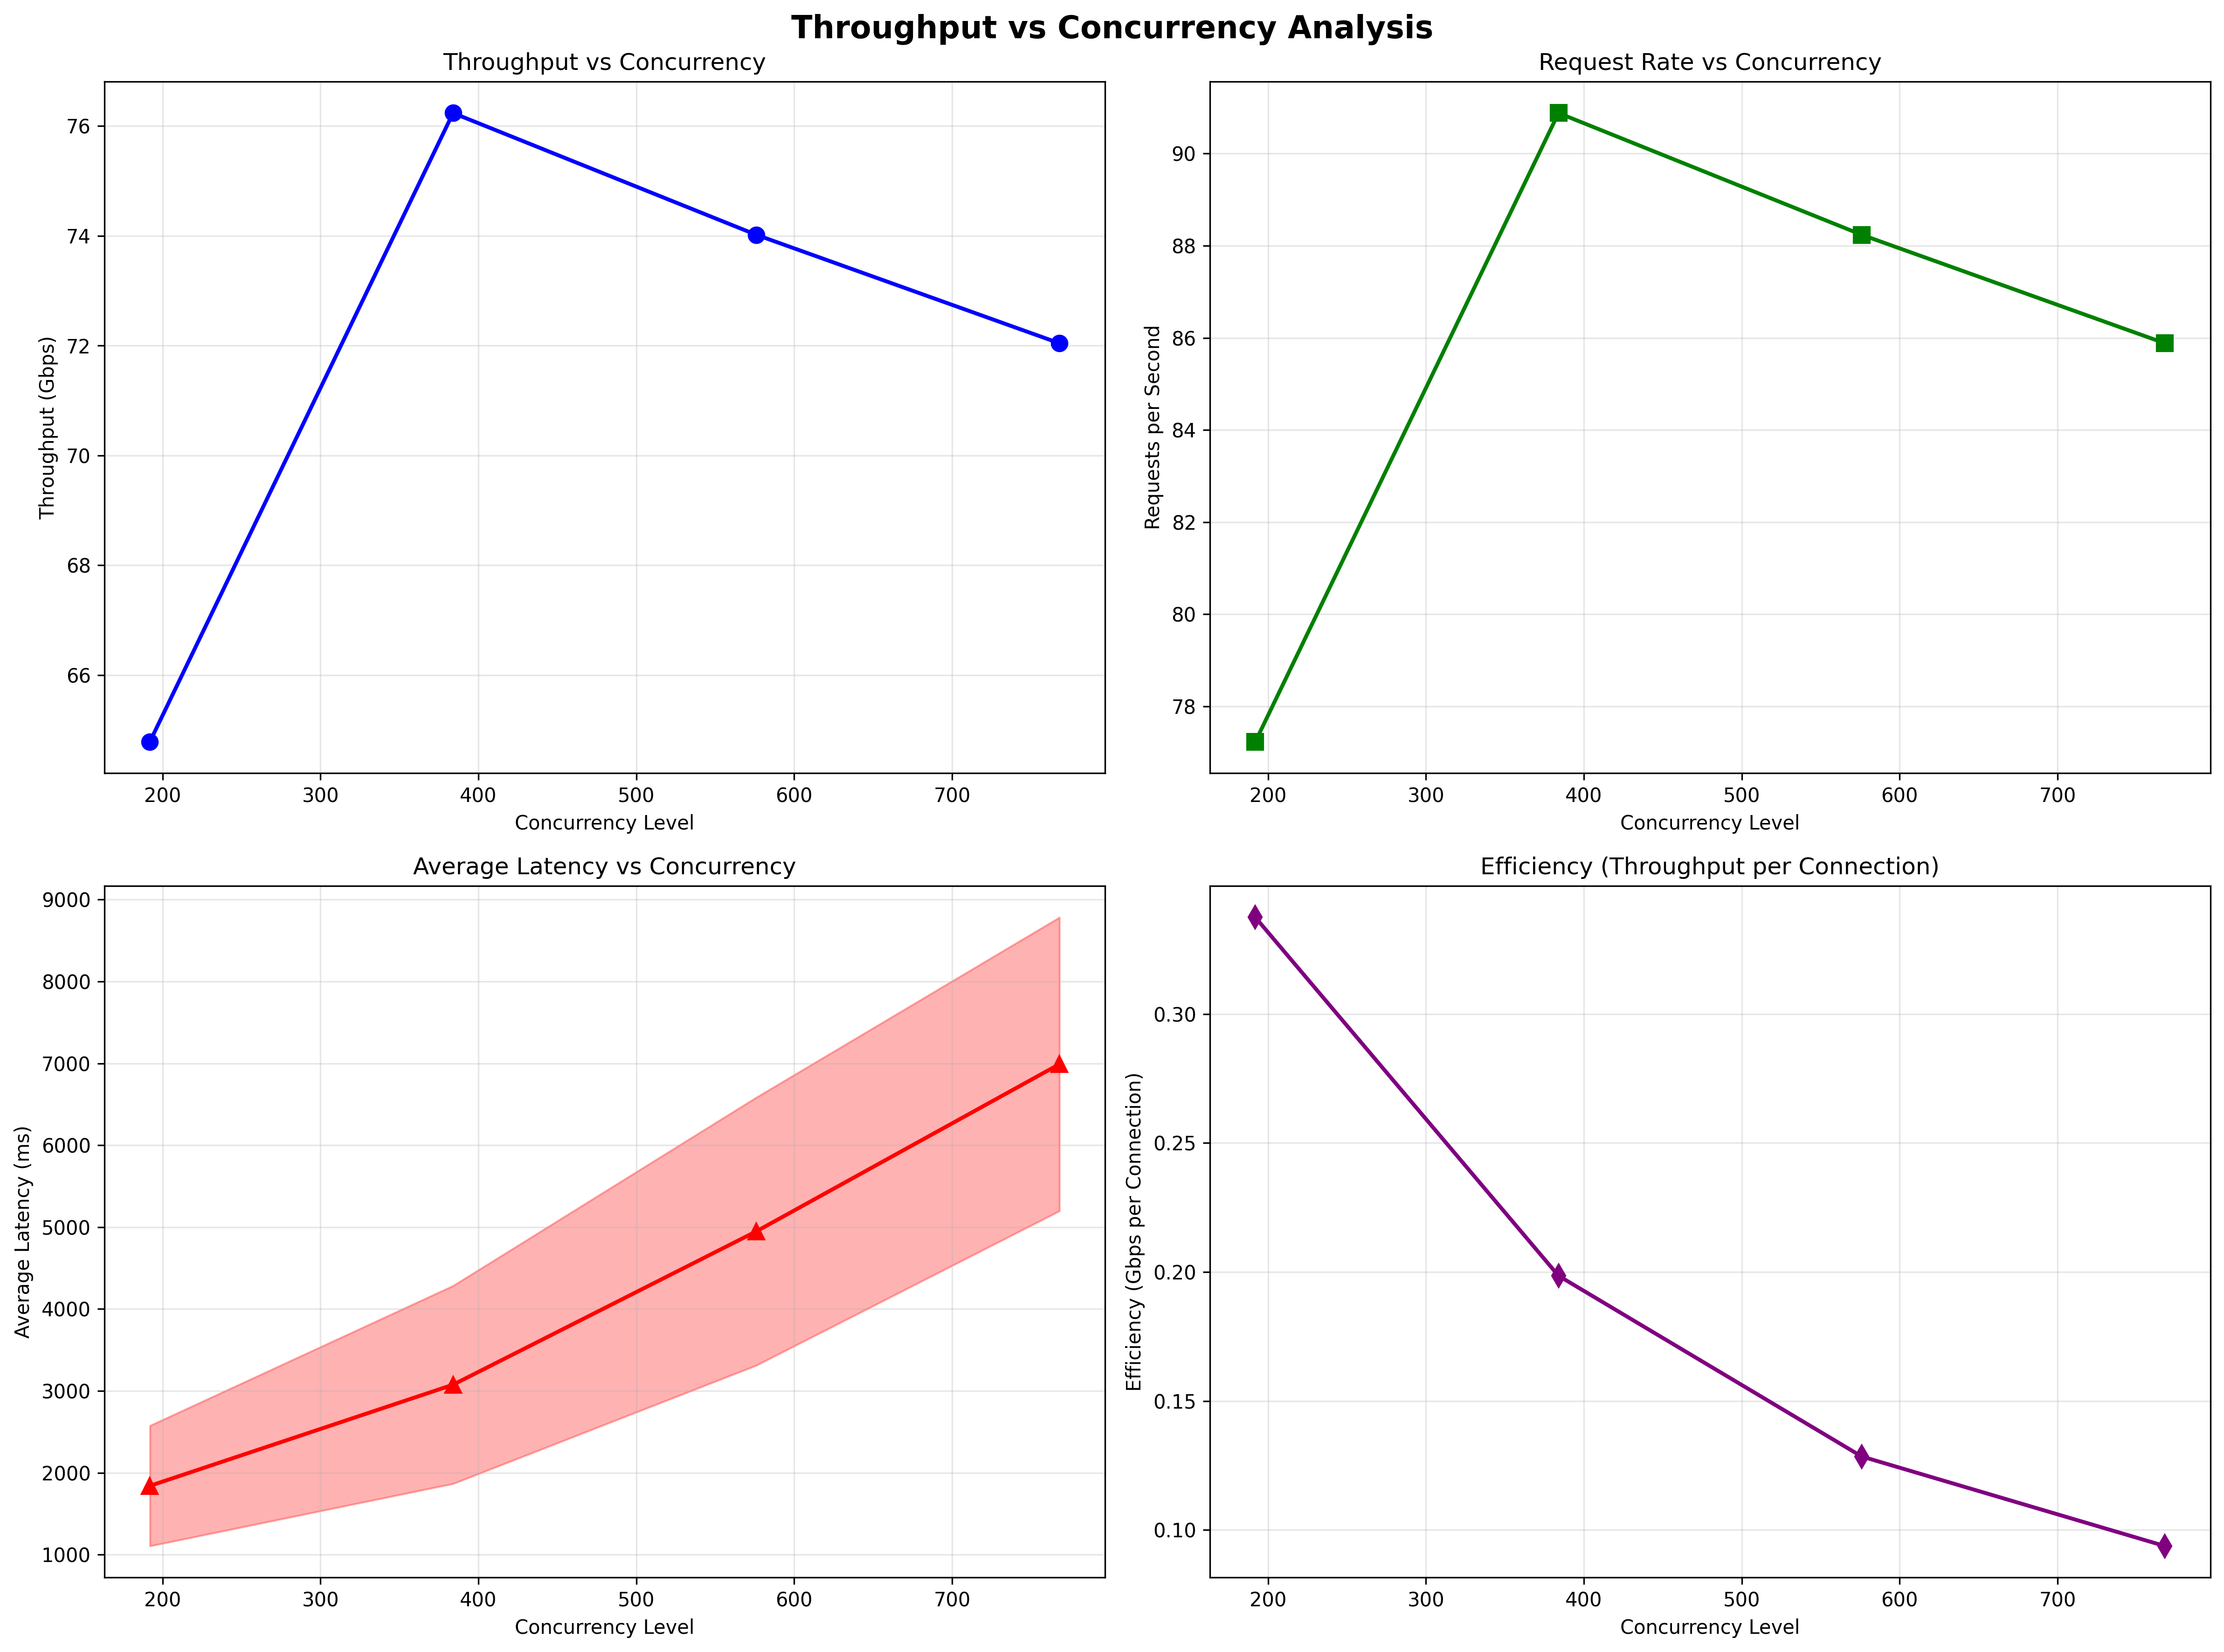
\includegraphics[width=\textwidth]{figures/c6in-16xlarge-throughput_vs_concurrency.png}
\caption{R2 throughput vs concurrency on c6in.16xlarge (100 Gbps): peak 78.4 Gbps at C384, declining to 72--75 Gbps at higher concurrency}
\label{fig:c6in16-throughput-vs-concurrency}
\end{figure}

\subsection{High Tier: 200 Gbps Instances}

The c6in.32xlarge baseline configuration (100 MB chunks, pipeline depth 3) achieved a peak throughput of 114.0 Gbps and average of 104.2 Gbps, representing 57\% utilization of the 200 Gbps interface. This represents the maximum system throughput observed in this study under the current client architecture. Network interface utilization remained at 55--57\% while CPU utilization sustained 90--99\% across all cores. CPU saturation is the directly observable constraint; however, the EC2 inbound IGW cap for this instance is also approximately 100~Gbps (50\% of 200~Gbps), coinciding with the measured ceiling---the two cannot be distinguished from client-side measurements alone.

The c6in.32xlarge-2 configuration (50 MB chunks, pipeline depth 6) achieved nearly identical aggregate throughput: 111.0 Gbps peak, 103.4 Gbps average. Figure~\ref{fig:c6in32-2-throughput-timeline} shows stable throughput progression across concurrency levels. The configuration change primarily impacted latency characteristics rather than aggregate throughput, confirming that the 110 Gbps ceiling is robust across different chunk size and pipeline depth settings.

\begin{figure}[H]
\centering
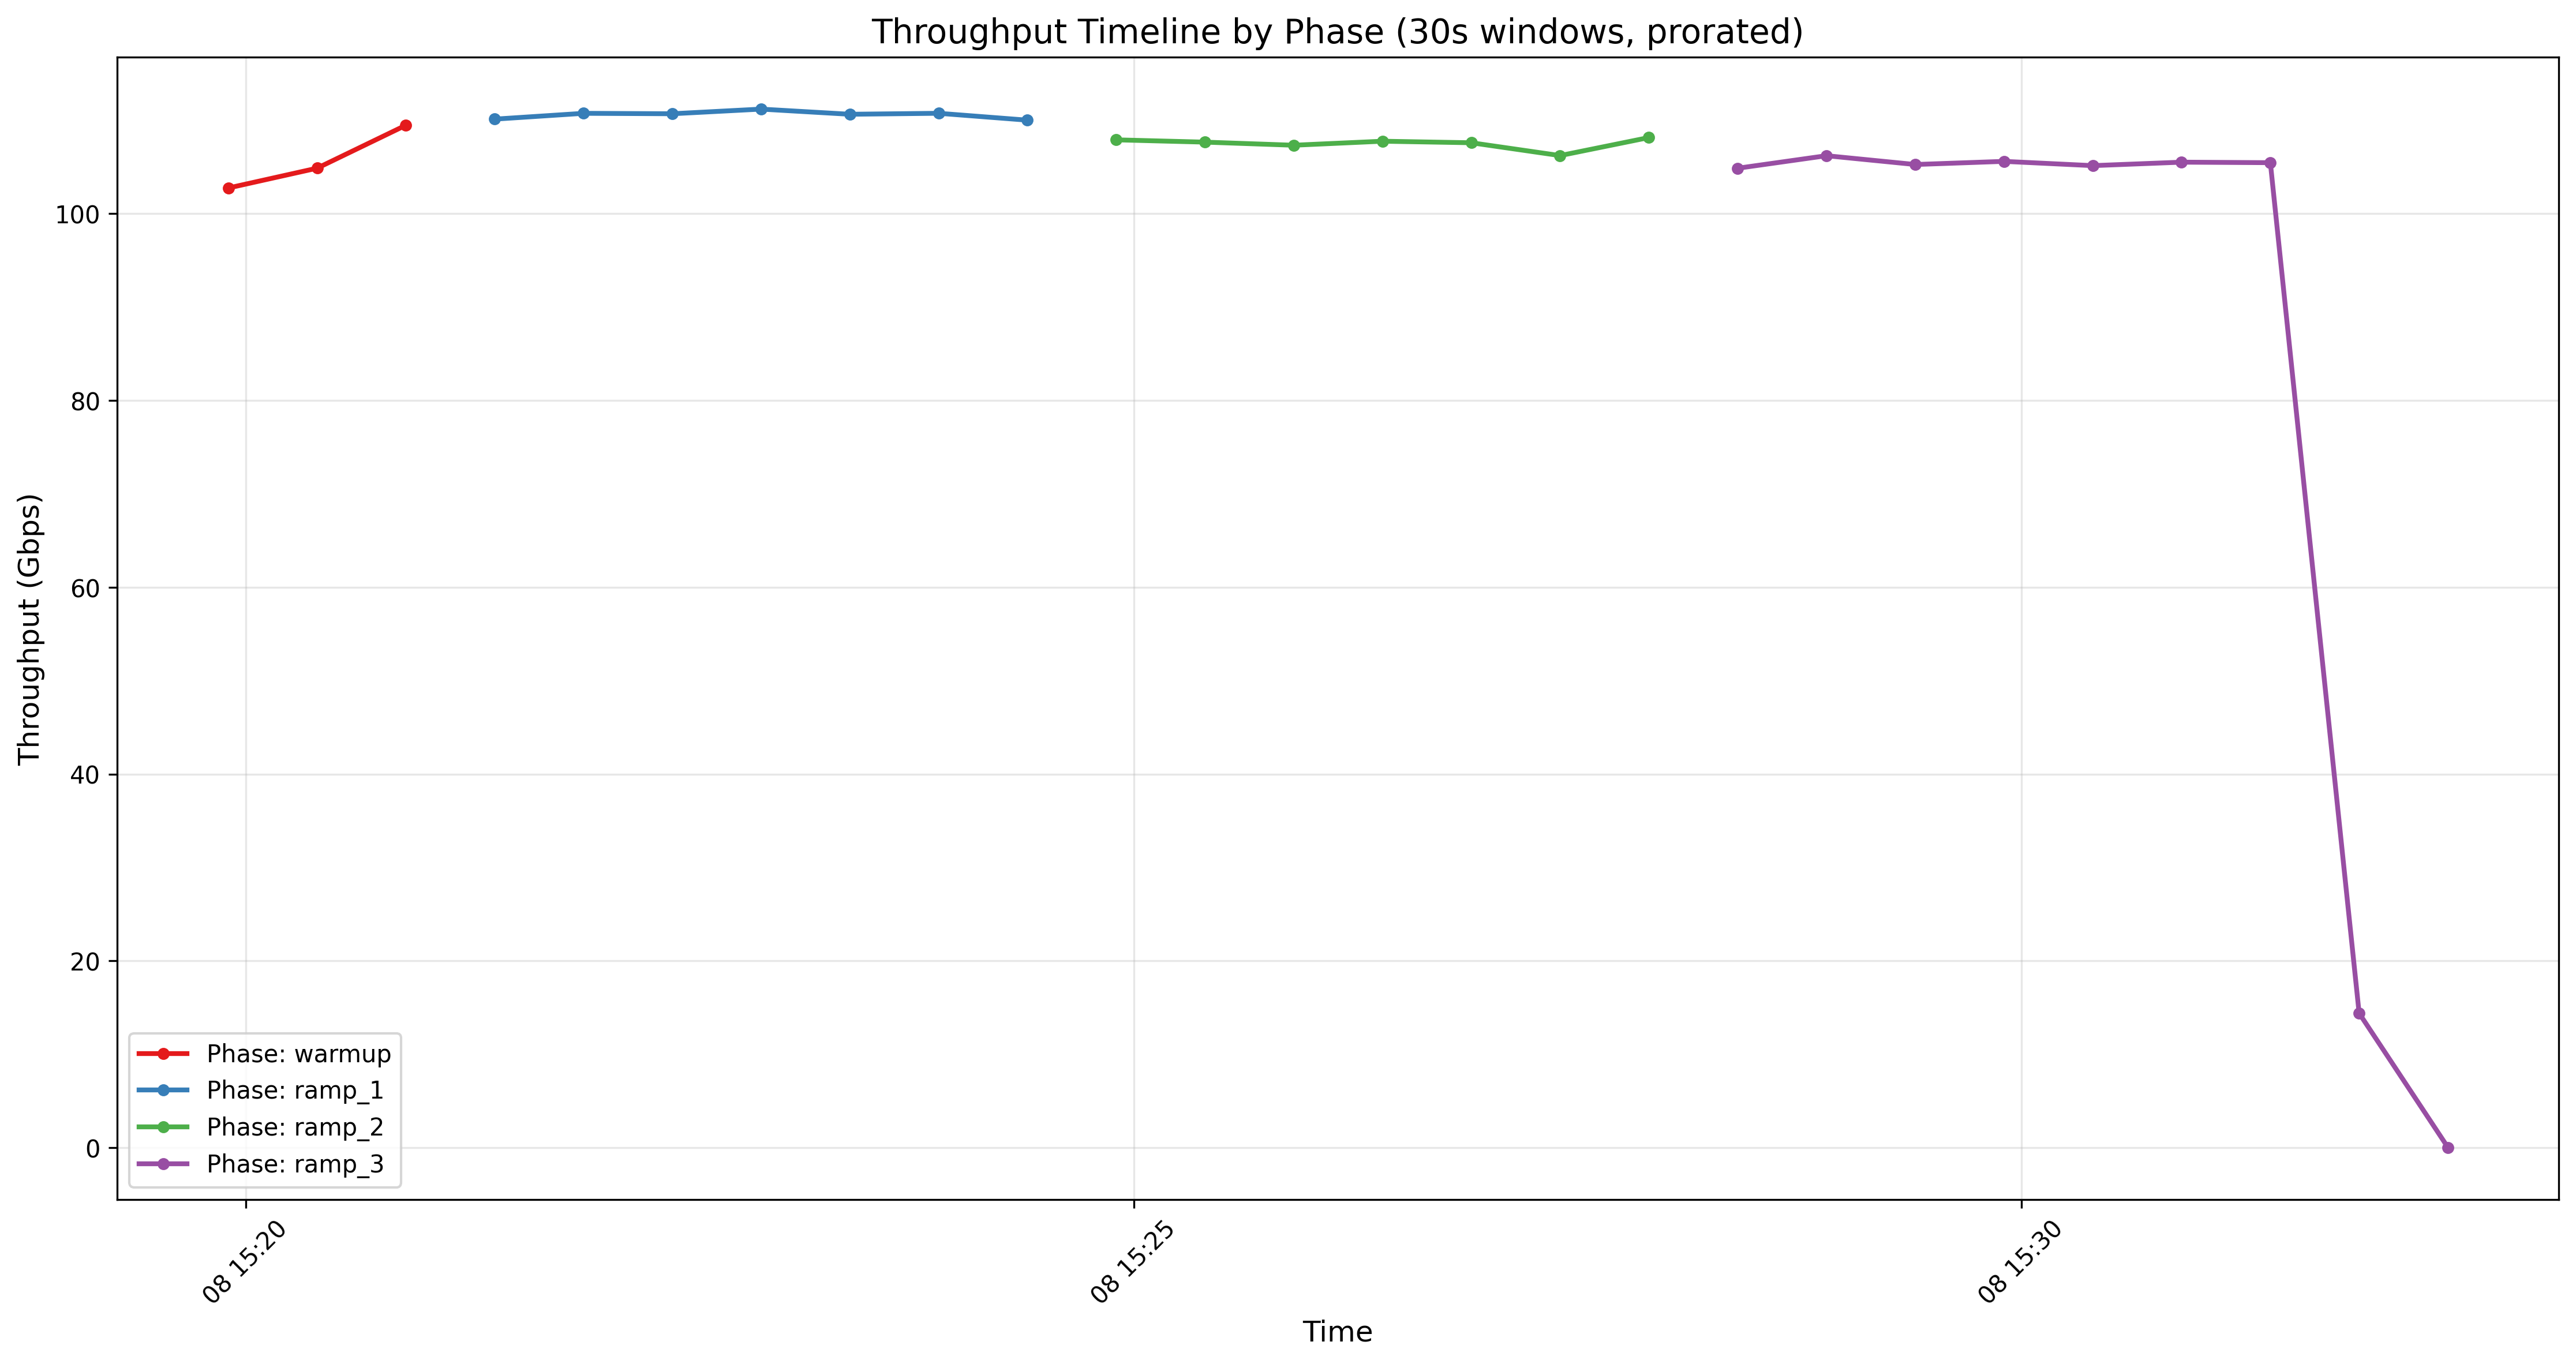
\includegraphics[width=\textwidth]{figures/c6in-32xlarge-2-throughput_timeline.png}
\caption{R2 throughput timeline on c6in.32xlarge-2 (50 MB chunks, 103 Gbps average)}
\label{fig:c6in32-2-throughput-timeline}
\end{figure}

Doubling vCPU count from 64 to 128 cores yielded only 1.42× throughput improvement (73.5 $\to$ 104.2 Gbps), confirming severe diminishing returns. The per-core throughput dropped from 1.15 Gbps/core (c6in.16xlarge) to 0.81 Gbps/core (c6in.32xlarge), indicating that coordination overhead, memory bandwidth saturation, and Python runtime inefficiencies increasingly constrain scaling at higher core counts.

The Frankfurt-deployed c6in.32xlarge-3 configuration achieved 89.1 Gbps average, representing a 14\% reduction compared to Stockholm's 103.4 Gbps. Peak throughput (108.3 Gbps) required 2× the concurrency (C1536) compared to Stockholm's peak at C768, suggesting differences in network path quality between AWS regions and Cloudflare's infrastructure, though without path-level measurements (e.g., traceroutes or RTT baselines to individual PoPs) the precise cause cannot be conclusively attributed.

The throughput difference is accompanied by a latency divergence that is not visible in median RTT alone. Table~\ref{tab:regional-latency} compares latency metrics for both regions at each region's respective peak concurrency. Median RTT is comparable (148~ms versus 142~ms), but the tail diverges sharply: RTT P95 is 83\% higher in Frankfurt (426~ms versus 233~ms), and total latency P95 is 78\% higher (5,793~ms versus 3,260~ms). The pattern is consistent with Frankfurt's routing path producing more variable queueing pressure under load: the typical request completes at a similar speed, but the tail is substantially longer, indicating that some fraction of requests encounter worse-than-average path conditions. This ``median holds, tail does not'' characteristic is a practically important distinction for latency-sensitive applications that care about percentile guarantees rather than only average throughput.

\begin{table}[H]
\centering
\caption{Regional latency comparison at respective peak concurrency: Stockholm (C768) vs Frankfurt (C1536). Same instance type, chunk size, and R2 bucket.}
\label{tab:regional-latency}
\small
\begin{tabular}{lcc}
\hline
\textbf{Metric} & \textbf{Stockholm (eu-north-1)} & \textbf{Frankfurt (eu-central-1)} \\
\hline
Average throughput         & 103.4 Gbps  & 89.1 Gbps (−14\%)          \\
Peak concurrency           & C768        & C1536 (2×)                 \\
RTT --- median             & 148 ms      & 142 ms                     \\
RTT --- P95                & 233 ms      & \textbf{426 ms} (+83\%)    \\
Total latency --- median   & 1{,}690 ms  & \textbf{2{,}809 ms} (+66\%)\\
Total latency --- P95      & 3{,}260 ms  & \textbf{5{,}793 ms} (+78\%)\\
\hline
\end{tabular}
\end{table}

The hpc7g.16xlarge instance (64 vCPUs, 200 Gbps EFA) achieved only 48.0 Gbps peak throughput (24\% utilization), with erratic behavior across concurrency levels. Despite having the same 64 vCPU count as c6in.16xlarge, throughput was 38\% lower. This confirms that EFA-equipped instances, optimized for low-latency cluster communication, are unsuitable for object storage benchmarking over the public internet.

\subsection{Answering RQ1: Can R2 Saturate High-Bandwidth Networks?}

Within the tested range, R2 delivered data without observable errors or throttling, and successfully saturated the 15~Gbps interface of the r8gd.4xlarge with 95\% efficiency. At higher bandwidths, CPU utilization held at 90--99\% while throughput plateaued at 40~Gbps (36 vCPUs), 78~Gbps (64 vCPUs), and 114~Gbps (128 vCPUs). For the 36- and 64-vCPU instances, the per-core CPU ceiling closely predicts the measured throughput and the measurements exceed the theoretical IGW caps, making CPU the more plausible binding constraint. For the 128-vCPU instance, the CPU ceiling ($\approx$102~Gbps) and the IGW cap (100~Gbps) predict nearly identical throughput, and the measured average of 104~Gbps marginally exceeds both---consistent with the estimates being approximate and with no enforcement of the IGW cap having been observed in these experiments, as with the other instances. Additionally, for the two ``up to'' instances (r5.xlarge and r8gd.4xlarge), the short test durations (14 and 11--13 minutes respectively) cannot confirm that throughput would remain stable under longer sustained load, as only the r8gd long-run experiments established a step-down at 28--37 minutes; the 32+ vCPU instances carry fixed bandwidth specifications and are not subject to this concern. Accordingly, this study cannot determine whether R2 can saturate interfaces above 15~Gbps without client-side or network-level constraints intervening first. These results establish a lower bound on R2 performance under large-object, single-client workloads and should not be interpreted as a full characterisation of system capacity.

The per-core ceiling ranges from approximately 1.5 Gbps at 4 vCPUs to 1.1 Gbps at 36--64 vCPUs and 0.8 Gbps at 128 vCPUs, reflecting increasing coordination overhead and Python runtime inefficiencies at higher parallelism. The maximum system throughput of 114 Gbps is within the same order of magnitude as the approximately 100 Gbps figure AWS documents for S3 from a single EC2 instance~\cite{aws-s3-performance}; since the client was the bottleneck in both cases, the similarity is consistent with shared client-side constraints rather than being informative about R2's or S3's actual backend capacity. All measured throughput values represent \textit{lower bounds} on R2's actual serving capacity; a client implemented in a compiled language would likely push this ceiling higher.

\section{Latency Characteristics Under Concurrency}\label{sec:latency-analysis}

Before examining results, it is important to clarify the difference between two latency metrics that are measured in the framework. 

\begin{itemize}
    \item \textbf{RTT (time-to-first-byte):} Time from issuing the \texttt{get\_object()} call to the moment the S3 client returns the response object --- i.e., when HTTP response headers arrive, \textit{before} any body bytes are read. This captures network round-trip and any server-side processing delay, independent of the amount of data requested.
    \item \textbf{Total latency:} Time from the same start point until \texttt{body.read()} completes --- i.e., when the full chunk has been received. Total latency = RTT + body transfer time. For a fixed throughput, larger chunks always produce proportionally higher total latency.
\end{itemize}

Because RTT is independent of chunk size, it provides a more direct signal about backend behaviour than total latency: elevated RTT may indicate queueing or processing delay at R2's backend, though it also captures TCP congestion and client-side scheduling effects and cannot cleanly isolate backend latency alone.

Table~\ref{tab:latency-summary} presents the overall latency statistics for all tested configurations. The reported P50, P95, and P99 values are percentile statistics computed over all requests across all concurrency levels. All tests achieved 100\% post-retry success rates; retry logging on r8gd.4xlarge-3 confirmed a retry rate of approximately 0.048\%.

\begin{table}[H]
\centering
\caption{R2 latency statistics: percentiles over all requests pooled across all concurrency levels}
\label{tab:latency-summary}
\small
\begin{tabular}{p{2.6cm}p{1.5cm}p{1.5cm}p{1.5cm}p{1.5cm}p{1.5cm}p{2.8cm}}
\hline
\textbf{Instance} & \textbf{Chunk} & \textbf{Duration} & \textbf{P50 (ms)} & \textbf{P95 (ms)} & \textbf{P99 (ms)} & \textbf{Concurrency Range} \\
\hline
r5.xlarge           & 100 MB & 0.24 hrs & 3,125  & 6,097  & 7,155  & 12--48 \\
r8gd.4xlarge        & 100 MB & 0.24 hrs & 5,566  & 11,536 & 13,793 & 48--192 \\
r8gd.4xlarge-2      & 100 MB & 1.19 hrs & 4,931  & 11,347 & 14,957 & 48--144 (steady C96) \\
r8gd.4xlarge-3      & 50 MB  & 1.19 hrs & 3,853  & 9,643  & 13,674 & 96--288 (steady C192) \\
c5n.9xlarge         & 100 MB & 0.19 hrs & 7,548  & 12,383 & 14,775 & 324--540 \\
c6in.16xlarge       & 100 MB & 0.25 hrs & 3,723  & 8,490  & 10,607 & 192--768 \\
hpc7g.16xlarge      & 100 MB & 0.20 hrs & 3,498  & 10,837 & 20,549 & 192--576 \\
c6in.32xlarge       & 100 MB & 0.23 hrs & 5,270  & 11,794 & 14,849 & 384--1536 \\
c6in.32xlarge-2     & 50 MB  & 0.21 hrs & 2,545  & 7,792  & 12,231 & 768--2304 \\
c6in.32xlarge-3     & 50 MB  & 0.20 hrs & 2,727  & 7,040  & 12,159 & 768--2304 \\
\hline
\end{tabular}
\end{table}

\subsection{Latency Growth with Concurrency}

Latency grows monotonically with concurrency across all tested instances. Figure~\ref{fig:c6in16-latency-over-time} illustrates the characteristic staircase pattern on c6in.16xlarge, where median latency increases from approximately 1.6 seconds at C192 to 6.8 seconds at C768 --- a 4.3× growth for a 4× increase in concurrency.

\begin{figure}[H]
\centering
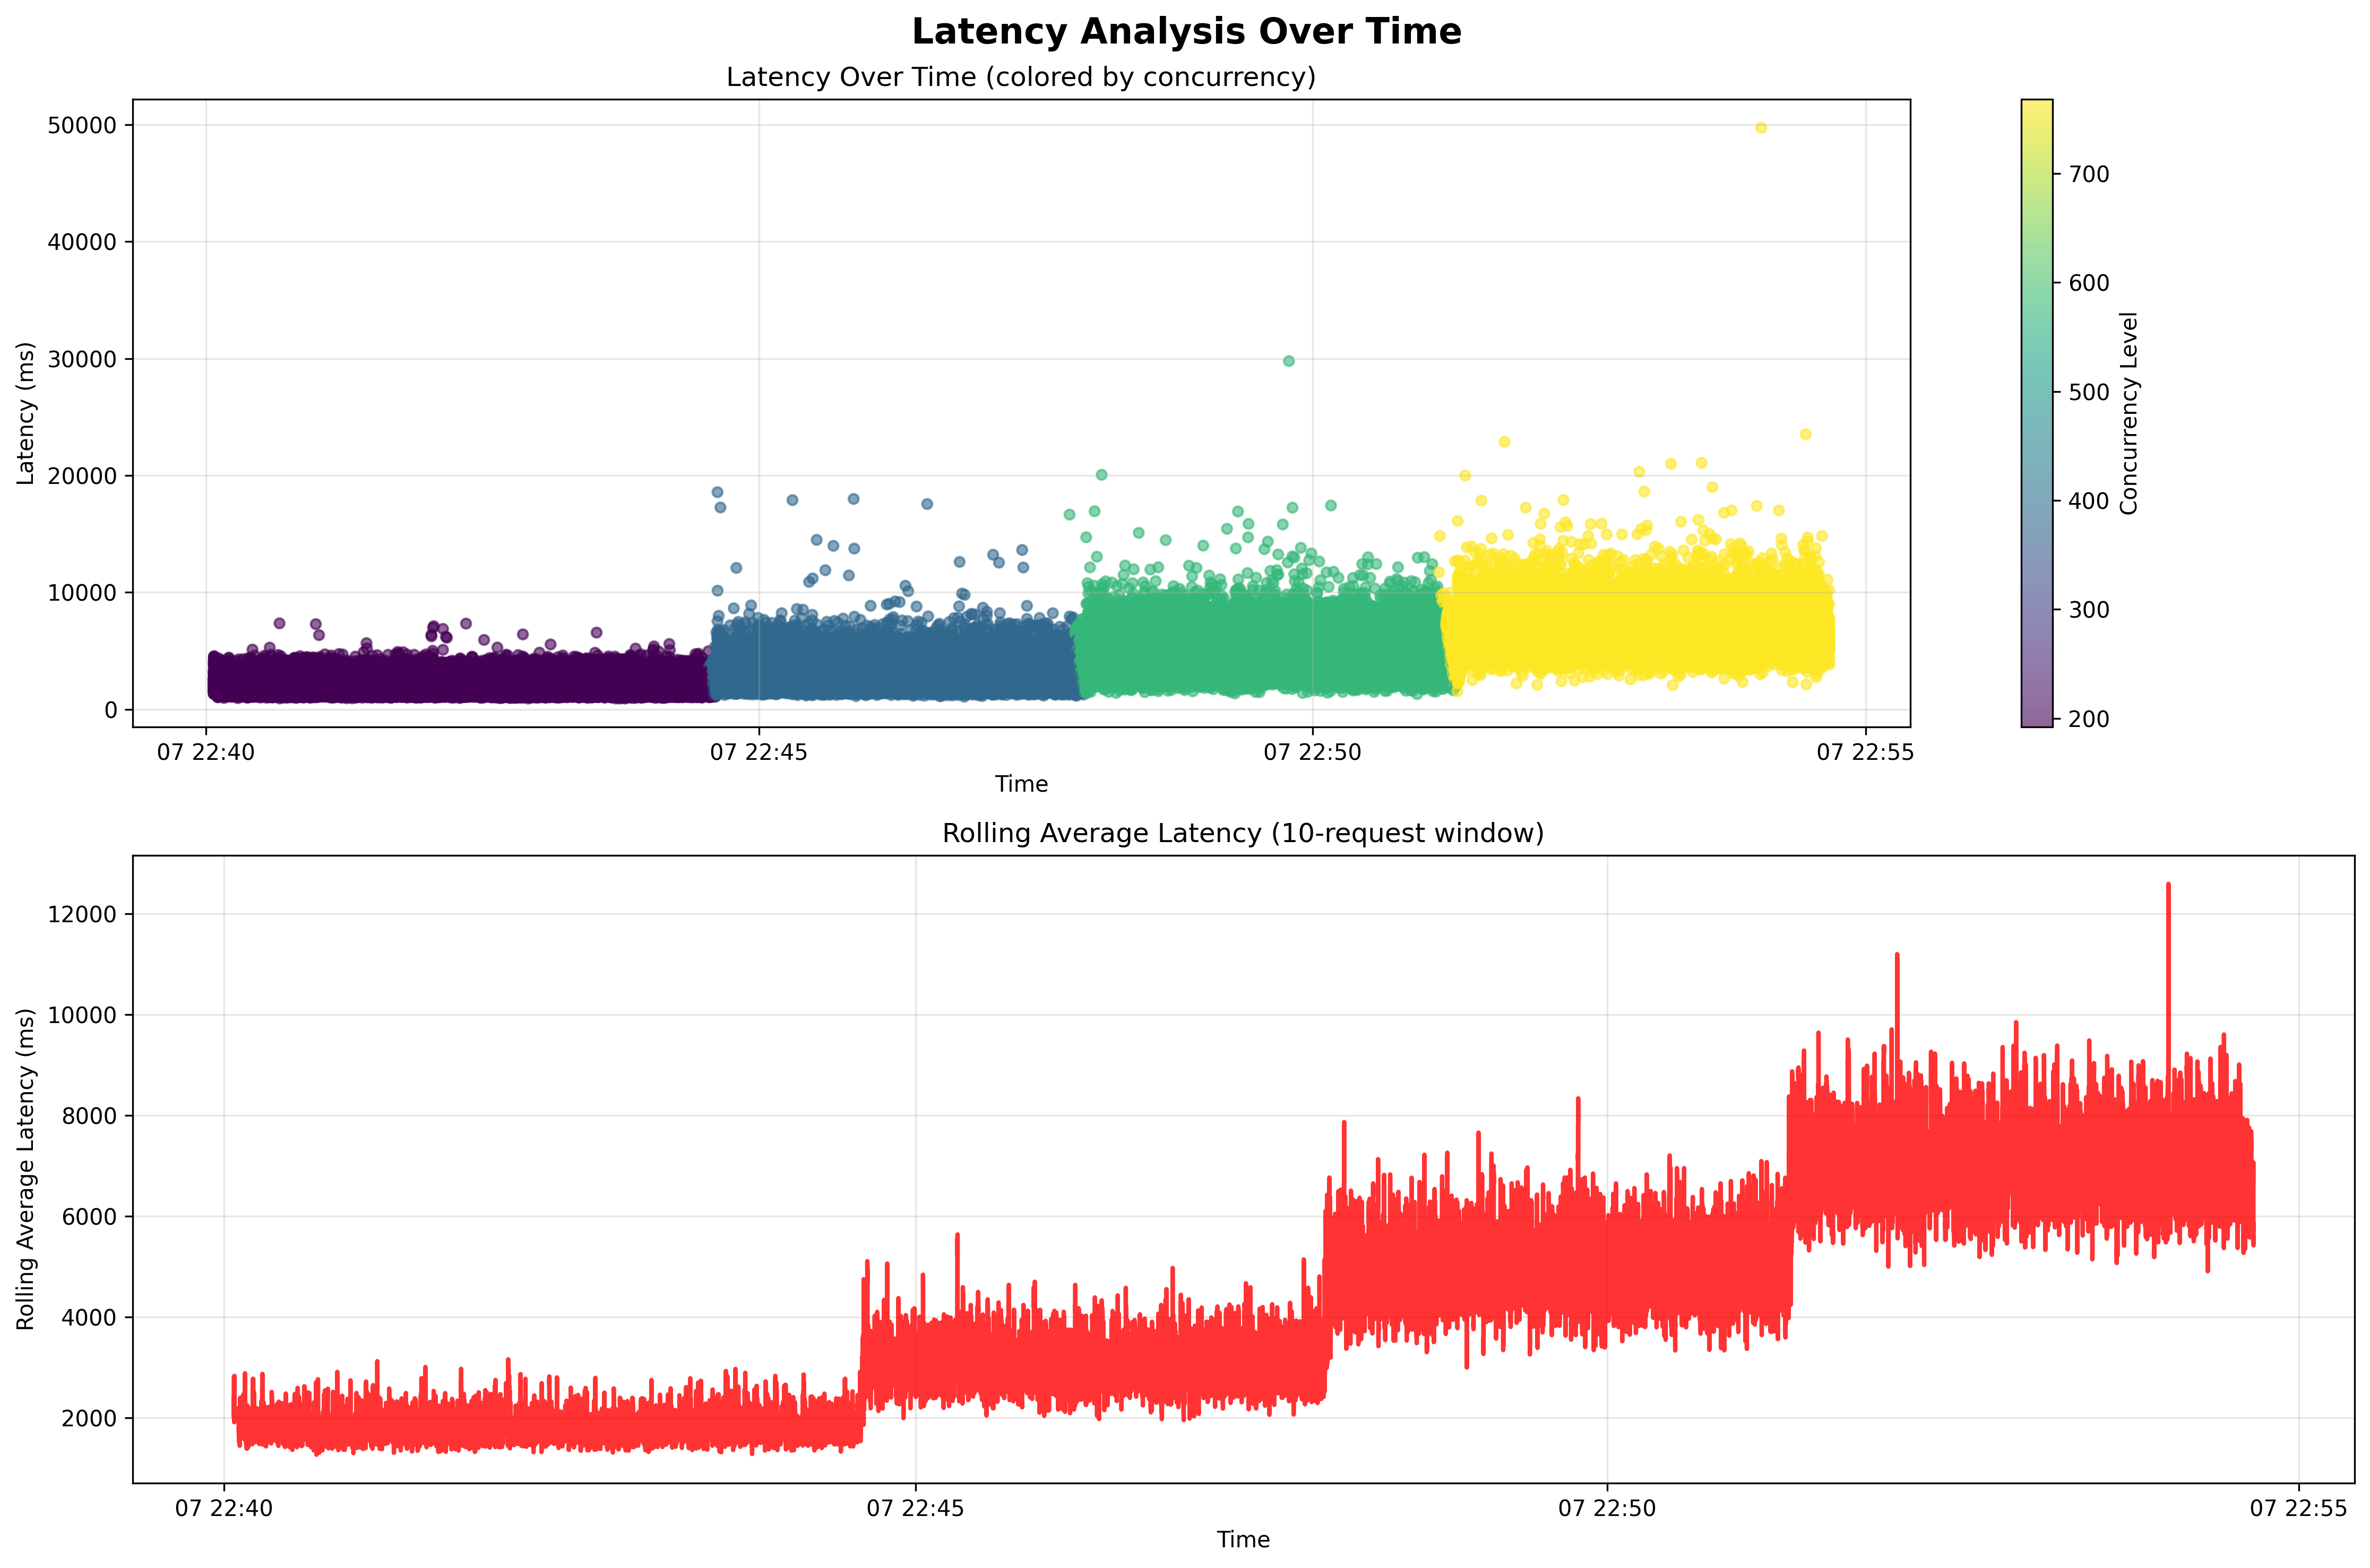
\includegraphics[width=\textwidth]{figures/c6in-16xlarge-latency_over_time.png}
\caption{Latency evolution over time on c6in.16xlarge: clear staircase steps at each concurrency transition}
\label{fig:c6in16-latency-over-time}
\end{figure}

The scaling is broadly proportional to offered load. On c6in.32xlarge-2, a 3× increase in concurrency (C768 $\to$ C2304) raised P99 from 4,182 ms to 15,337 ms --- a 3.7× increase. This is consistent with the queueing dynamics described by Little's Law ($L = \lambda W$), which predicts that when throughput $\lambda$ is saturated, mean latency $W$ grows linearly with the number of in-flight requests $L$~\cite{little2011}. Little's Law is a descriptive identity rather than a causal model; the observed proportionality is consistent with a queueing interpretation but other factors (TCP congestion, server-side scheduling) may contribute and cannot be isolated from client-side measurements alone. Su et al.\ \cite{su2017predicting} applied queueing-theory models specifically to cloud object storage, demonstrating that latency percentiles follow predictable patterns once a system approaches capacity. The system degrades gradually rather than collapsing, which is important for predictable capacity planning.

\subsection{RTT Analysis: Backend Behaviour Indicators}

Because RTT is measured before body transfer, it more directly reflects R2's request handling than total latency does, though it also captures TCP path variability and client-side scheduling effects. Due to the absence of server-side visibility, all latency attributions in this section are inferences from client-side observations; causal claims remain speculative and should be read as hypotheses consistent with the data rather than verified explanations. Figure~\ref{fig:c6in16-rtt} shows RTT on c6in.16xlarge across its concurrency levels. At C192, RTT stays near 120 ms; by C768 it reaches a median of 4,323 ms. At peak concurrency on c6in.32xlarge (100 MB configuration), RTT reached 5,925 ms, representing 62\% of total mean latency (9,546 ms). Since RTT captures all pre-transfer delay---including TCP congestion, kernel scheduling, client-side queueing, and any backend processing---this suggests that queueing or congestion pressure somewhere in the request path, rather than data transfer itself, accounts for the majority of elapsed time under saturation.

\begin{figure}[H]
\centering
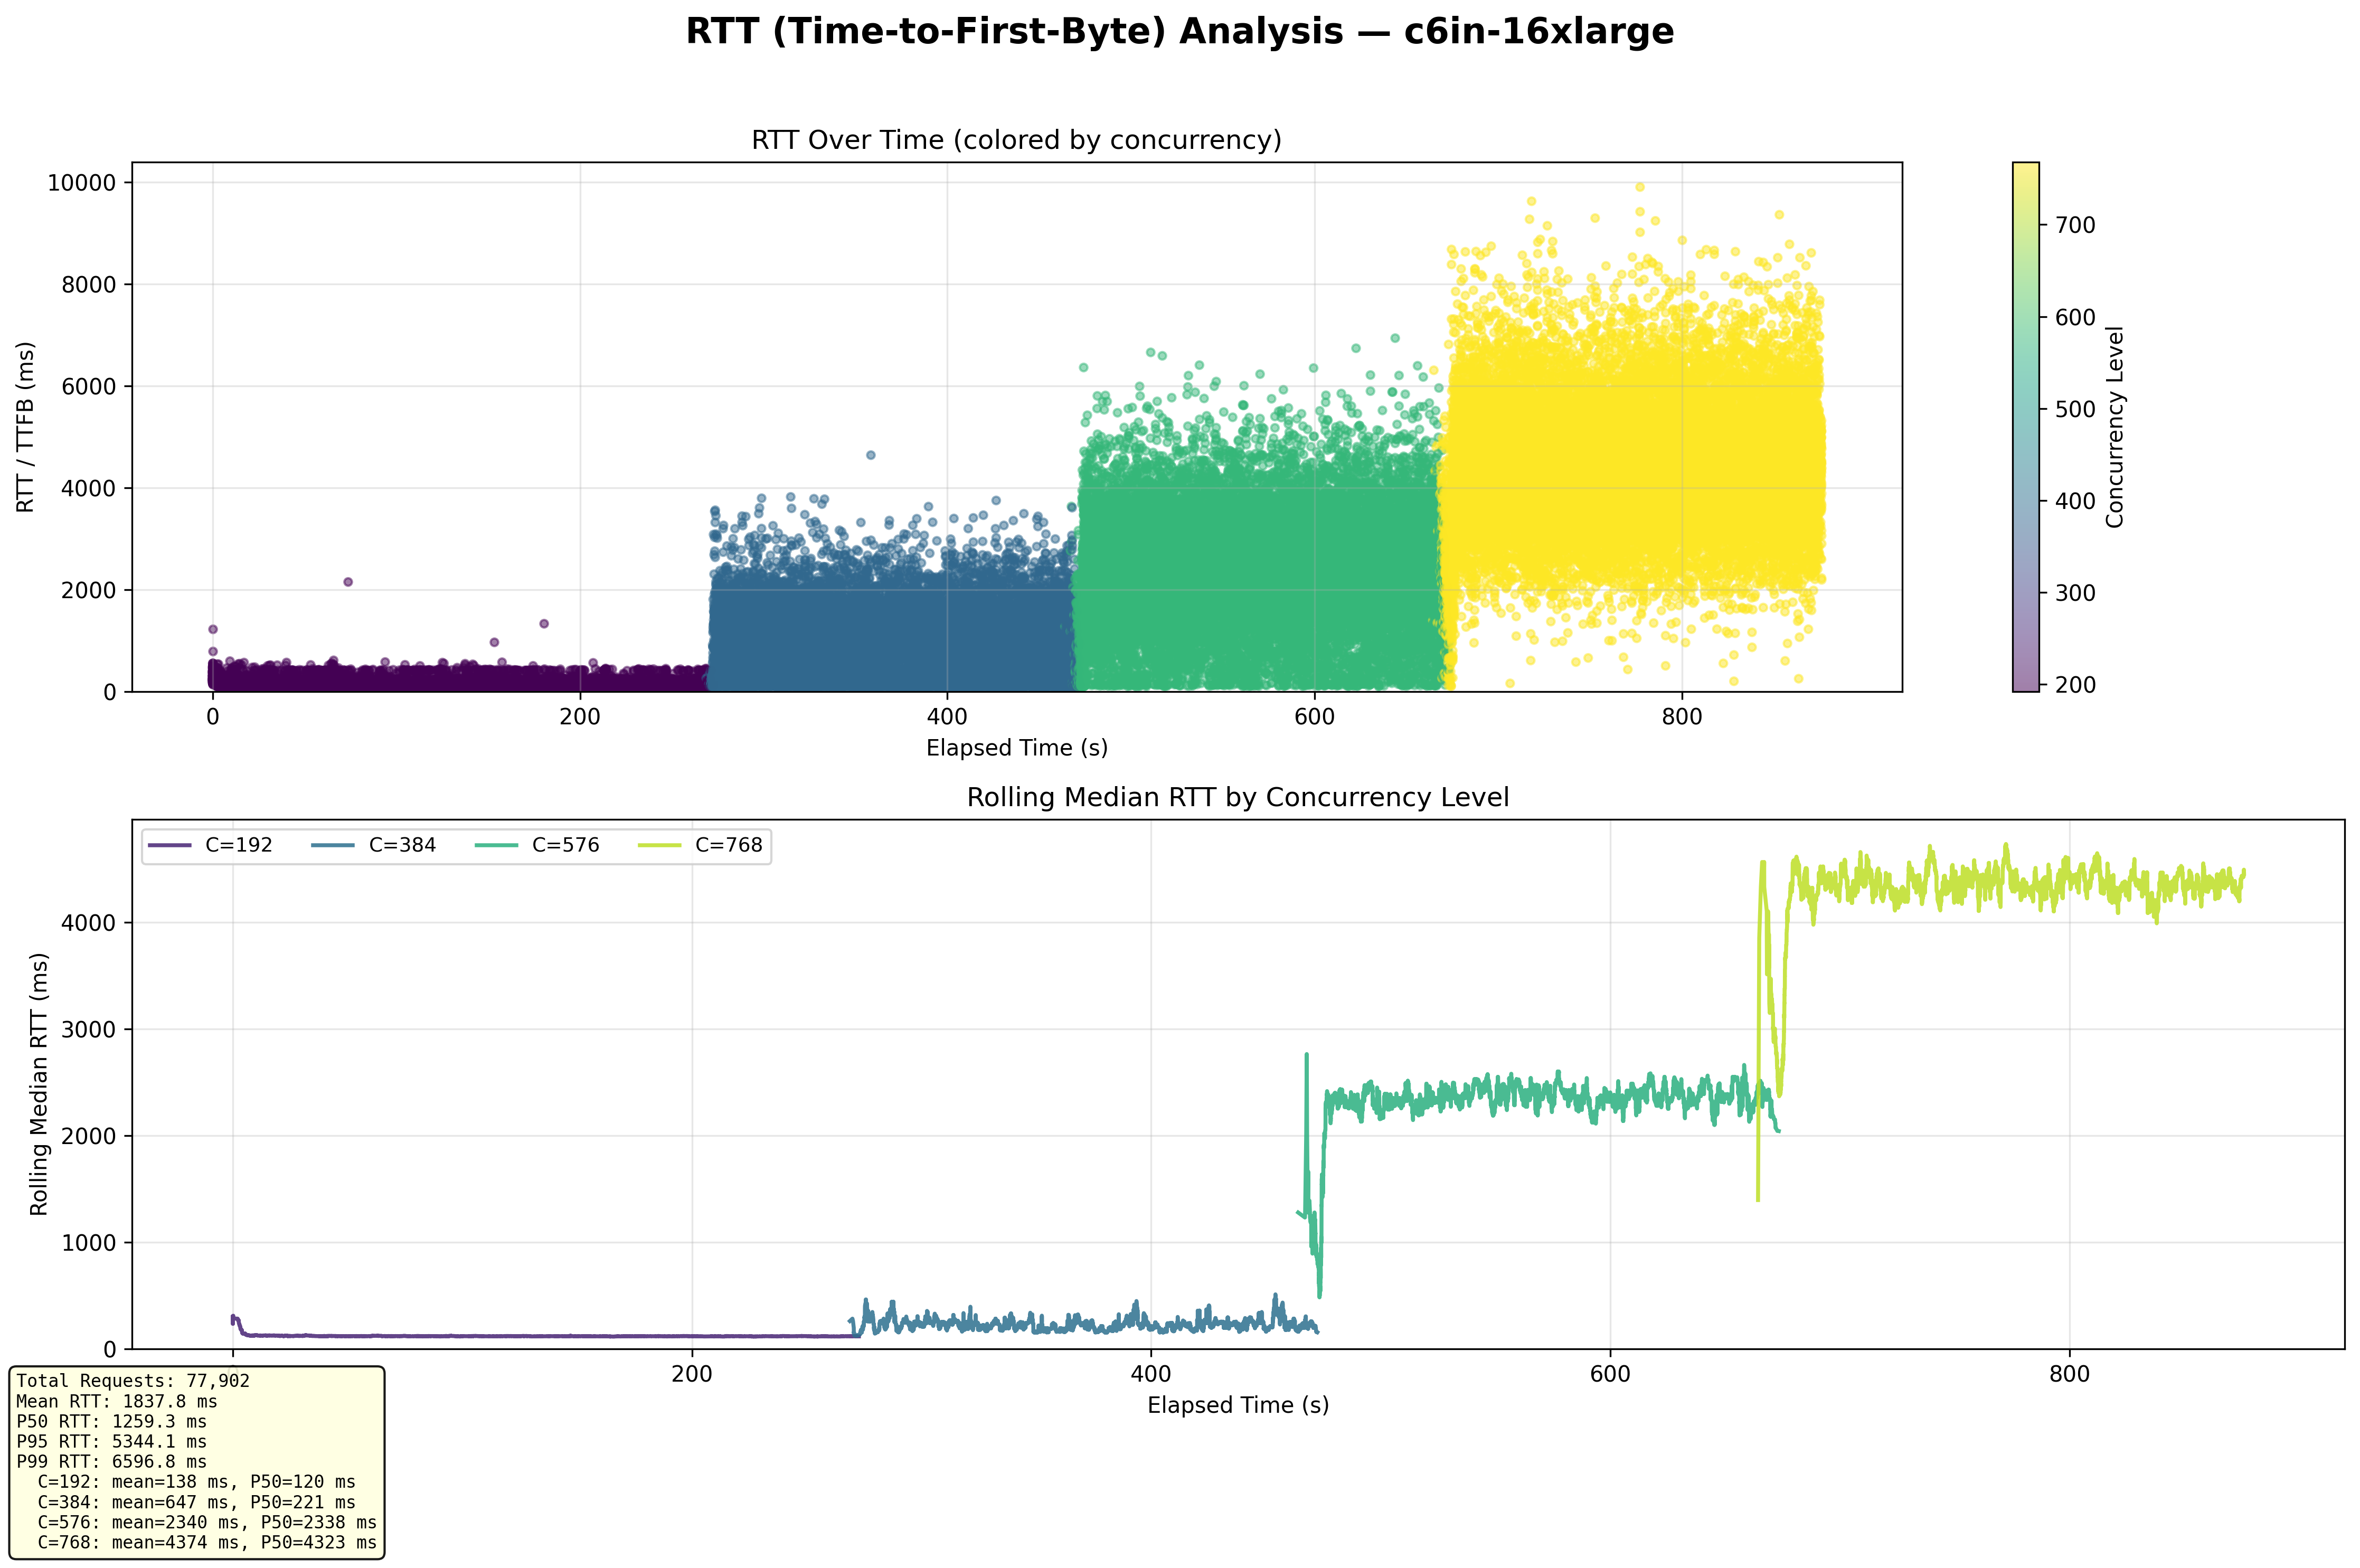
\includegraphics[width=\textwidth]{figures/c6in-16xlarge-rtt_over_time.png}
\caption{RTT on c6in.16xlarge: 120 ms at C192 growing to 4,323 ms median at C768}
\label{fig:c6in16-rtt}
\end{figure}

AWS documentation reports S3 first-byte latency of 100--200 ms for large objects under normal operating conditions~\cite{aws-s3-performance}. R2 operates in a comparable range at low concurrency (120--200 ms RTT). This is corroborated by direct measurements on the same c6in.16xlarge instance (collected with an earlier framework version; see Section~\ref{sec:limitations}): at low concurrency S3 total latency was approximately 1,100 ms P50 for 100 MB objects, consistent with 100--200 ms first-byte latency plus roughly 900 ms transfer time at the available per-connection bandwidth. Both systems therefore exhibit comparable backend responsiveness when not under saturation pressure.

\subsection{Configuration Impact: Chunk Size and Concurrency}

The c6in.32xlarge instance was tested with two configurations to isolate the effect of chunk size on backend behaviour. Table~\ref{tab:chunk-size-comparison} compares results at matching concurrency (C768):

\begin{table}[H]
\centering
\caption{Chunk size comparison on c6in.32xlarge (Stockholm, C768)}
\label{tab:chunk-size-comparison}
\begin{tabular}{p{2.6cm}p{2.4cm}p{2.4cm}p{1.8cm}p{1.8cm}p{2.2cm}}
\hline
\textbf{Configuration} & \textbf{Throughput} & \textbf{Avg Latency} & \textbf{P99} & \textbf{Avg RTT} & \textbf{RTT fraction} \\
\hline
100 MB / p=3 & 109.3 Gbps & 4,209 ms & 9,445 ms & 838 ms  & 20\% \\
50 MB / p=6  & 110.7 Gbps & 1,875 ms & 4,182 ms & 163 ms  & 9\%  \\
\hline
\end{tabular}
\end{table}

Aggregate throughput is nearly identical (109--111 Gbps). The 50 MB configuration naturally shows lower total latency since a smaller chunk transfers faster at the same throughput. The non-obvious result is the RTT: 163 ms vs 838 ms at C768, and 251 ms vs 5,925 ms at peak concurrency (Figure~\ref{fig:c6in32-rtt-comparison}). Since RTT is independent of chunk size, this difference is consistent with the 50~MB configuration generating substantially less queueing pressure somewhere in the request path at equal aggregate throughput.

\begin{figure}[H]
\centering
\begin{minipage}{0.49\textwidth}
    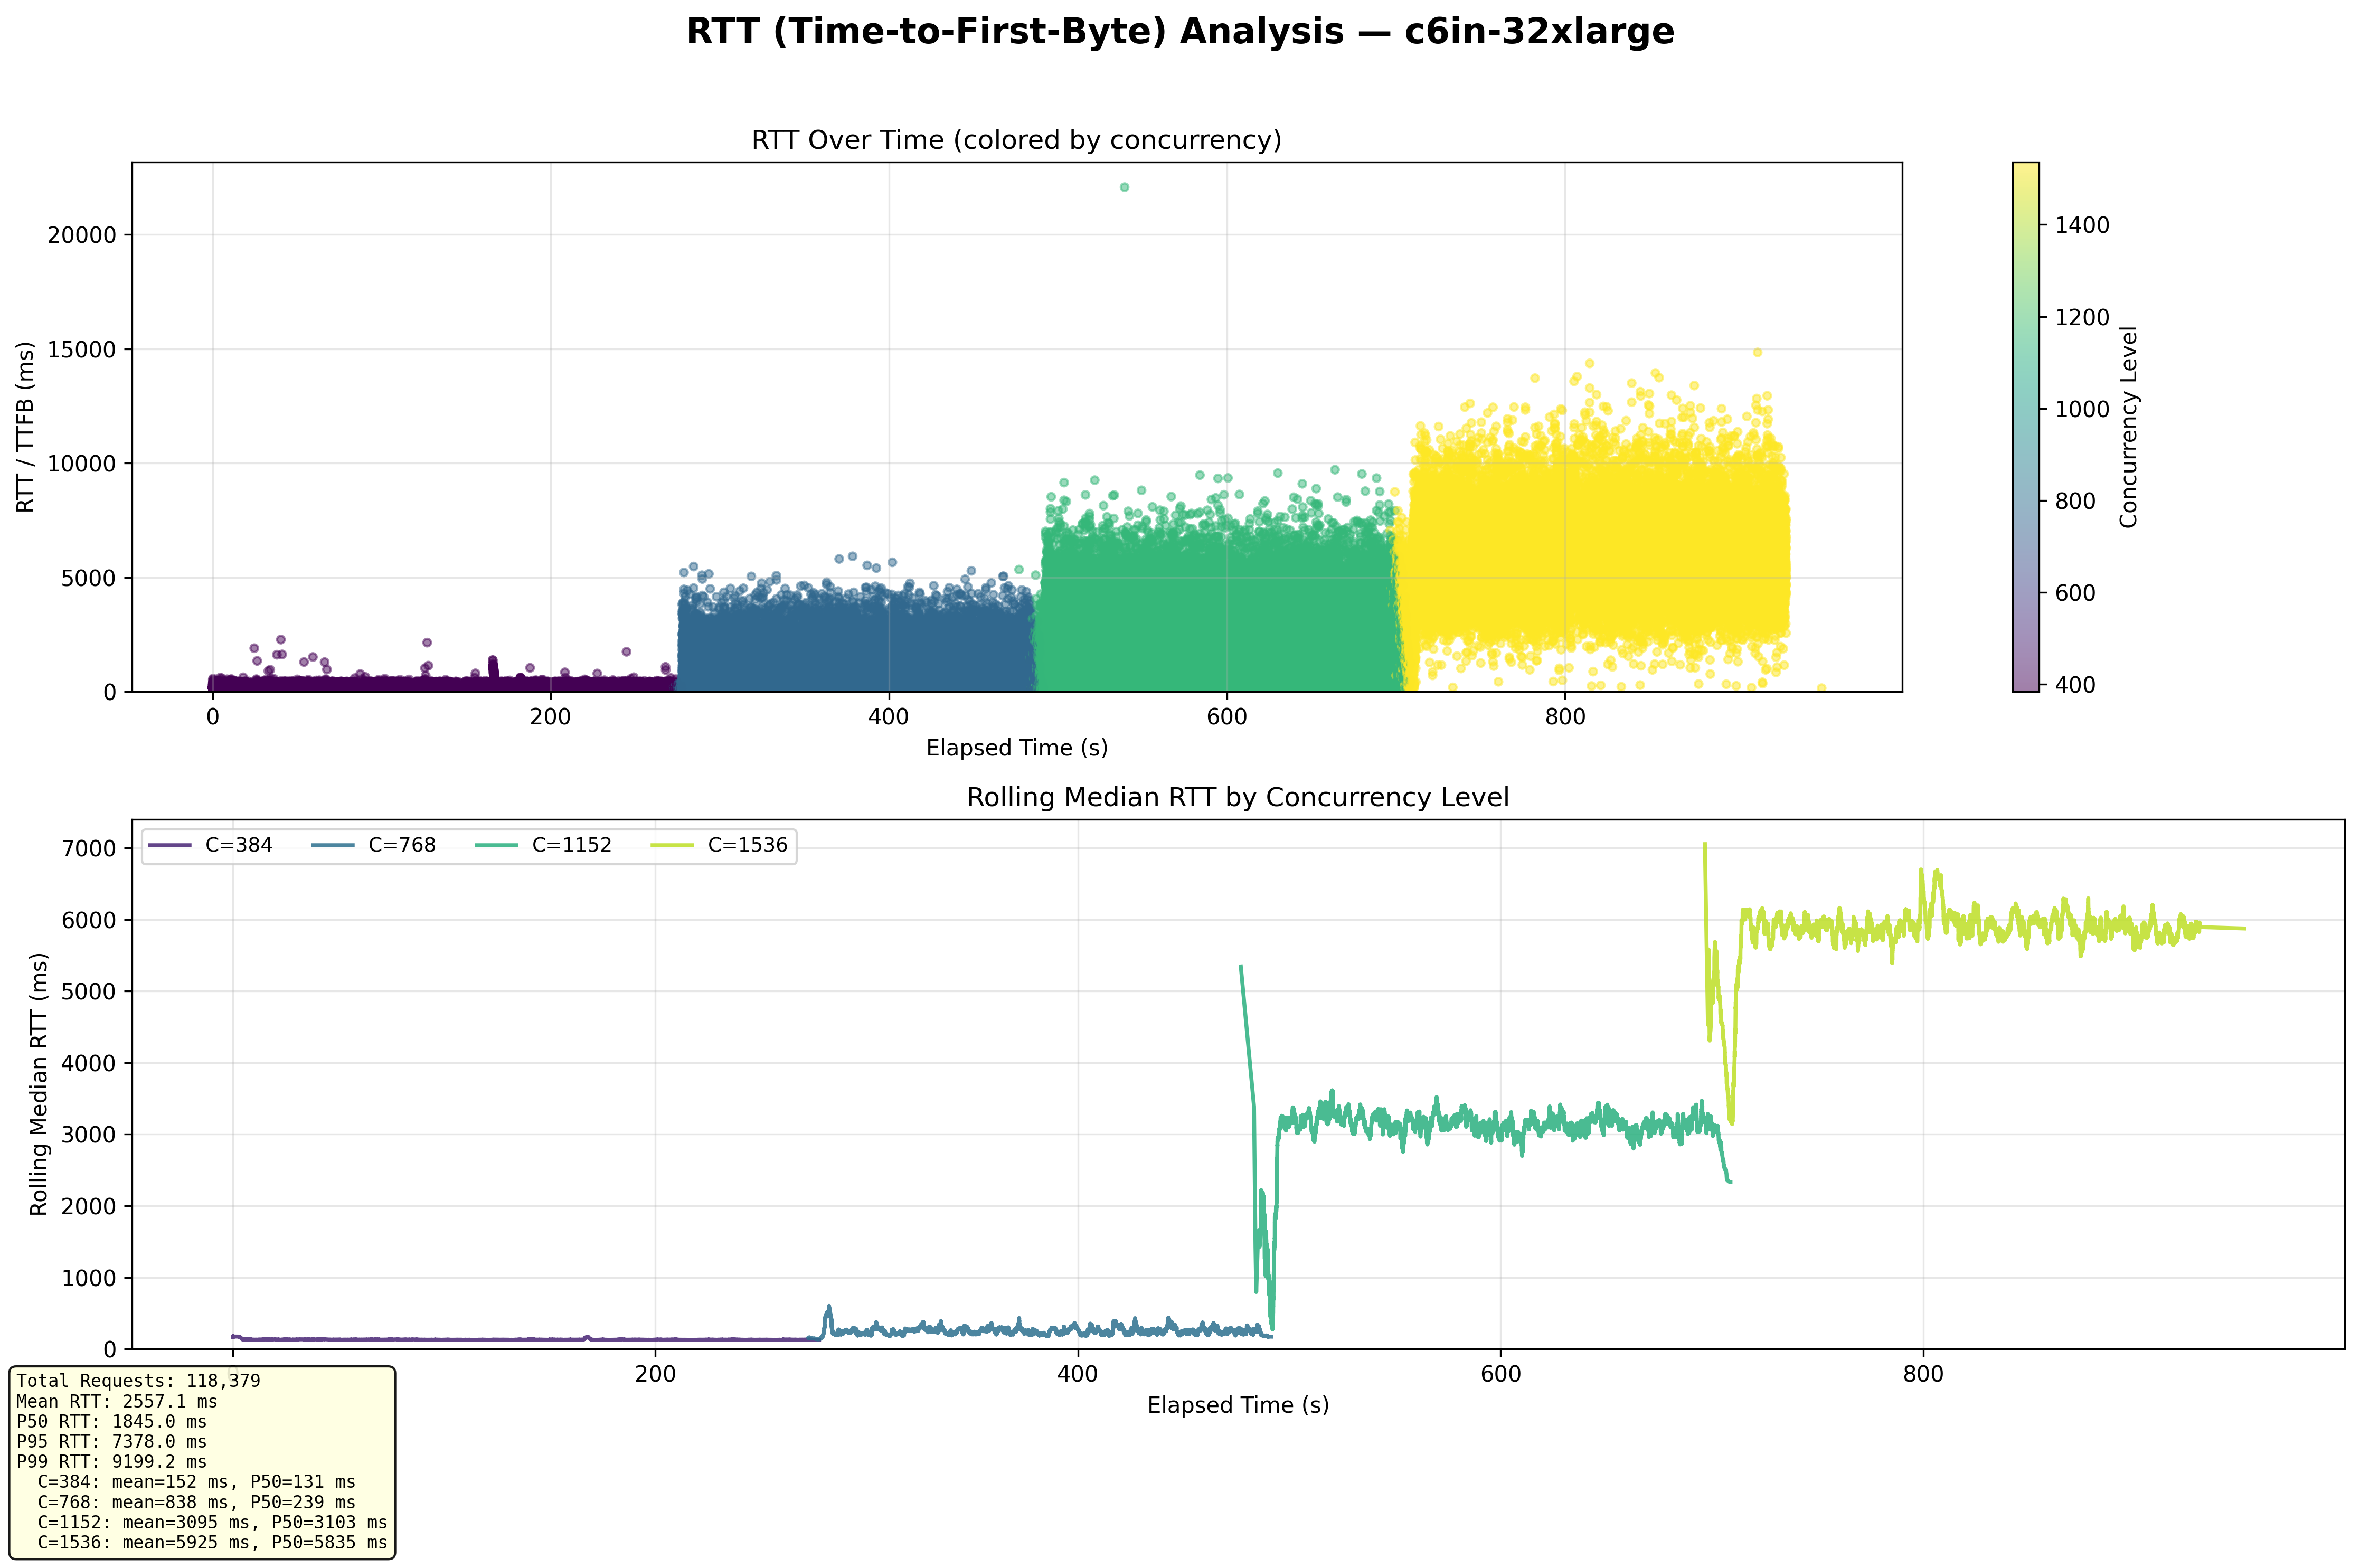
\includegraphics[width=\textwidth]{figures/c6in-32xlarge-rtt_over_time.png}
\end{minipage}
\hfill
\begin{minipage}{0.49\textwidth}
    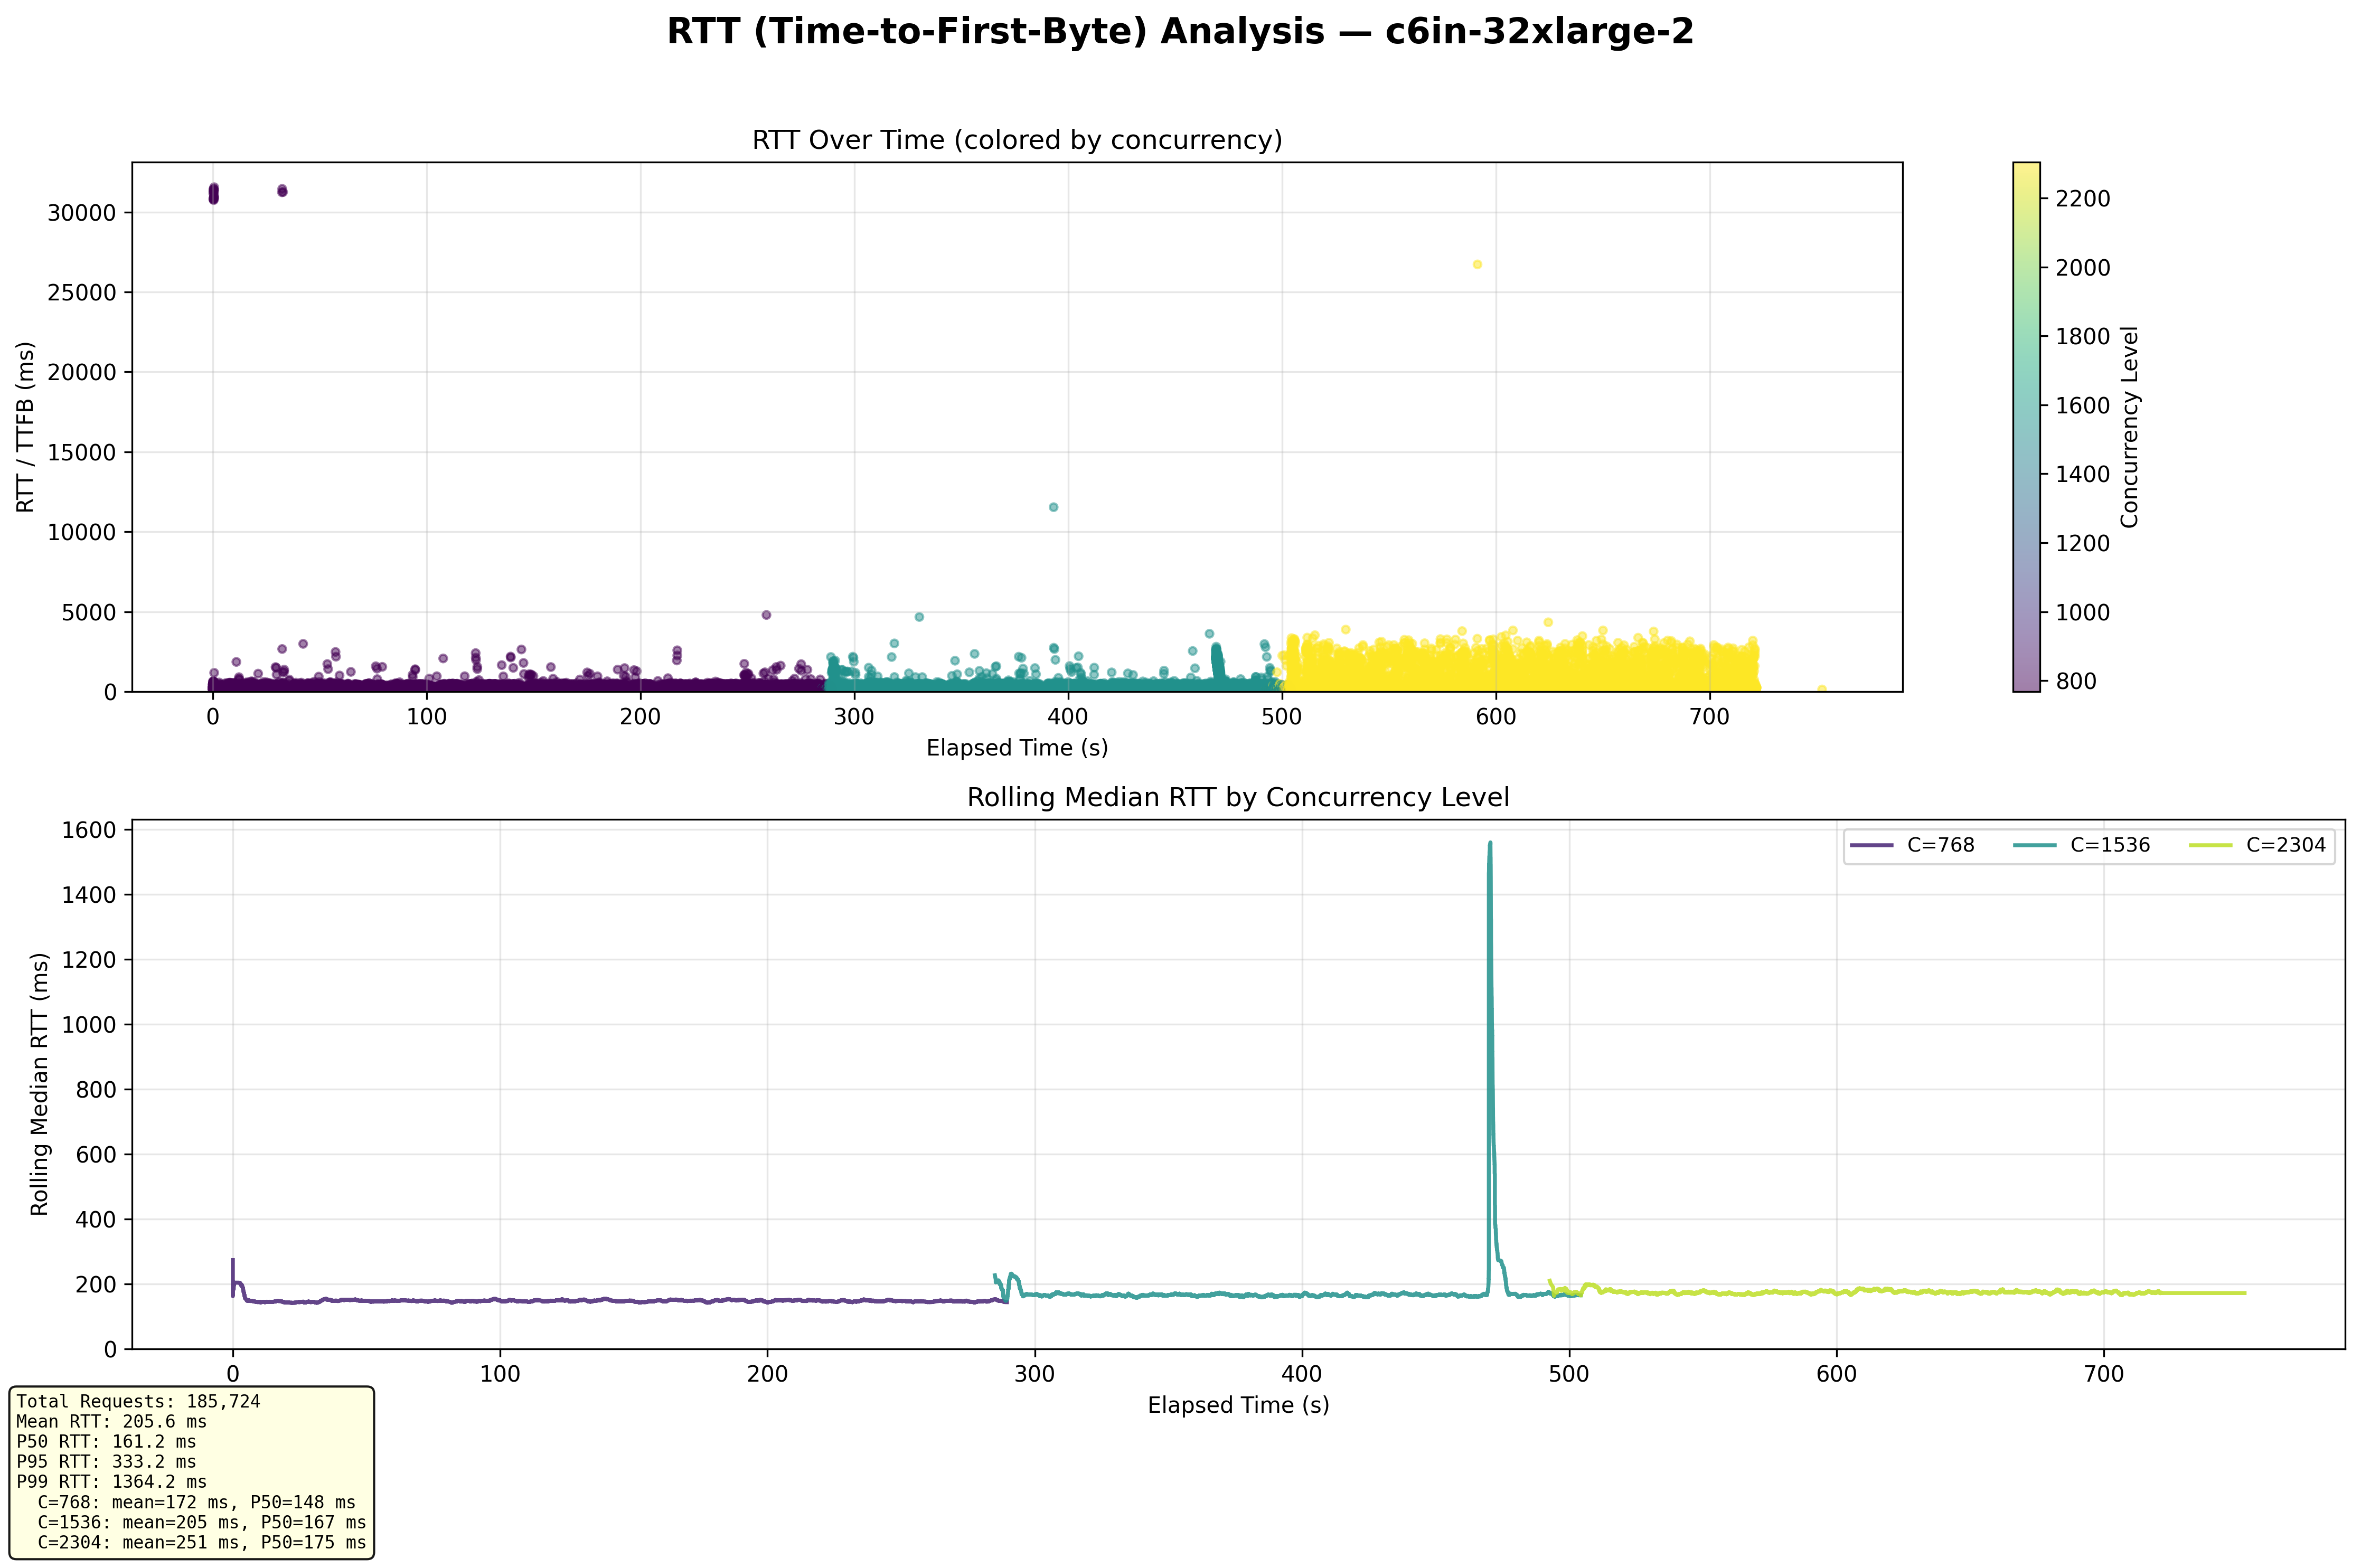
\includegraphics[width=\textwidth]{figures/c6in-32xlarge-2-rtt_over_time.png}
\end{minipage}
\caption{RTT: 100 MB chunks (left) vs 50 MB chunks (right) on c6in.32xlarge Stockholm. Same throughput ($\approx$103 Gbps), RTT at peak concurrency drops from 5,925 ms to 251 ms.}
\label{fig:c6in32-rtt-comparison}
\end{figure}

The most parsimonious explanation consistent with the data is the effect of per-request service time on queue depth. Under a queueing-theory model, the number of in-flight requests is proportional to both arrival rate and per-request service time; smaller 50~MB chunks complete in roughly half the time of 100~MB chunks at the same per-connection bandwidth, which would reduce steady-state queue depth at equal concurrency and lower the wait time before service begins. A contribution from the difference in HTTP pipeline depth (p=6 vs p=3) cannot be ruled out---pipelining depth affects how requests are batched within a single TCP connection and may influence scheduling along the path---but the magnitude of the RTT reduction (5$\times$ at peak concurrency) is more consistent with a queueing-depth effect than a scheduling artifact. The exact location of the queue (client buffer, network, or R2 backend) cannot be determined without server-side instrumentation. Regardless of mechanism, the practical conclusion is clear: for latency-sensitive workloads at high concurrency, smaller request granularity is strongly preferable to larger chunks, even when aggregate throughput is identical.

\subsection{Steady-State Latency: Bandwidth Cliff and Paired Configuration Comparison}

Two r8gd.4xlarge experiments were run for approximately 1.19 hours each, using paired configurations with the same chunk$\times$pipeline product to isolate the effect of chunk size at matched aggregate load. r8gd.4xlarge-2 used 100 MB chunks with pipeline depth 3 (config B), ramping from C=48 to a steady-state of C=96. r8gd.4xlarge-3 used 50 MB chunks with pipeline depth 6 (config A), ramping from C=96 to a steady-state of C=192. Both configurations produce approximately the same total in-flight data volume (100 MB $\times$ 3 $\approx$ 50 MB $\times$ 6), enabling a direct comparison of chunk granularity effects.

Both runs share the same defining pattern: throughput holds at 14.2--14.3 Gbps during an initial elevated period, then drops permanently to approximately 7.1 Gbps. Figure~\ref{fig:r8gd-steady-state} shows this for r8gd.4xlarge-2. The cliff is a hard step-function transition---no gradual degradation, no recovery---consistent with the network I/O credit mechanism documented by AWS for ``up to'' bandwidth instances~\cite{aws-ec2-network-bandwidth}: once the initial allocation is consumed under sustained demand, the available bandwidth reverts to its underlying sustained level. The transition occurred at approximately 28 minutes into steady-state on run 2 and at approximately 37 minutes on run 3; the post-cliff throughput of $\approx$7.1 Gbps remained stable for the remainder of both runs.

\begin{figure}[H]
\centering
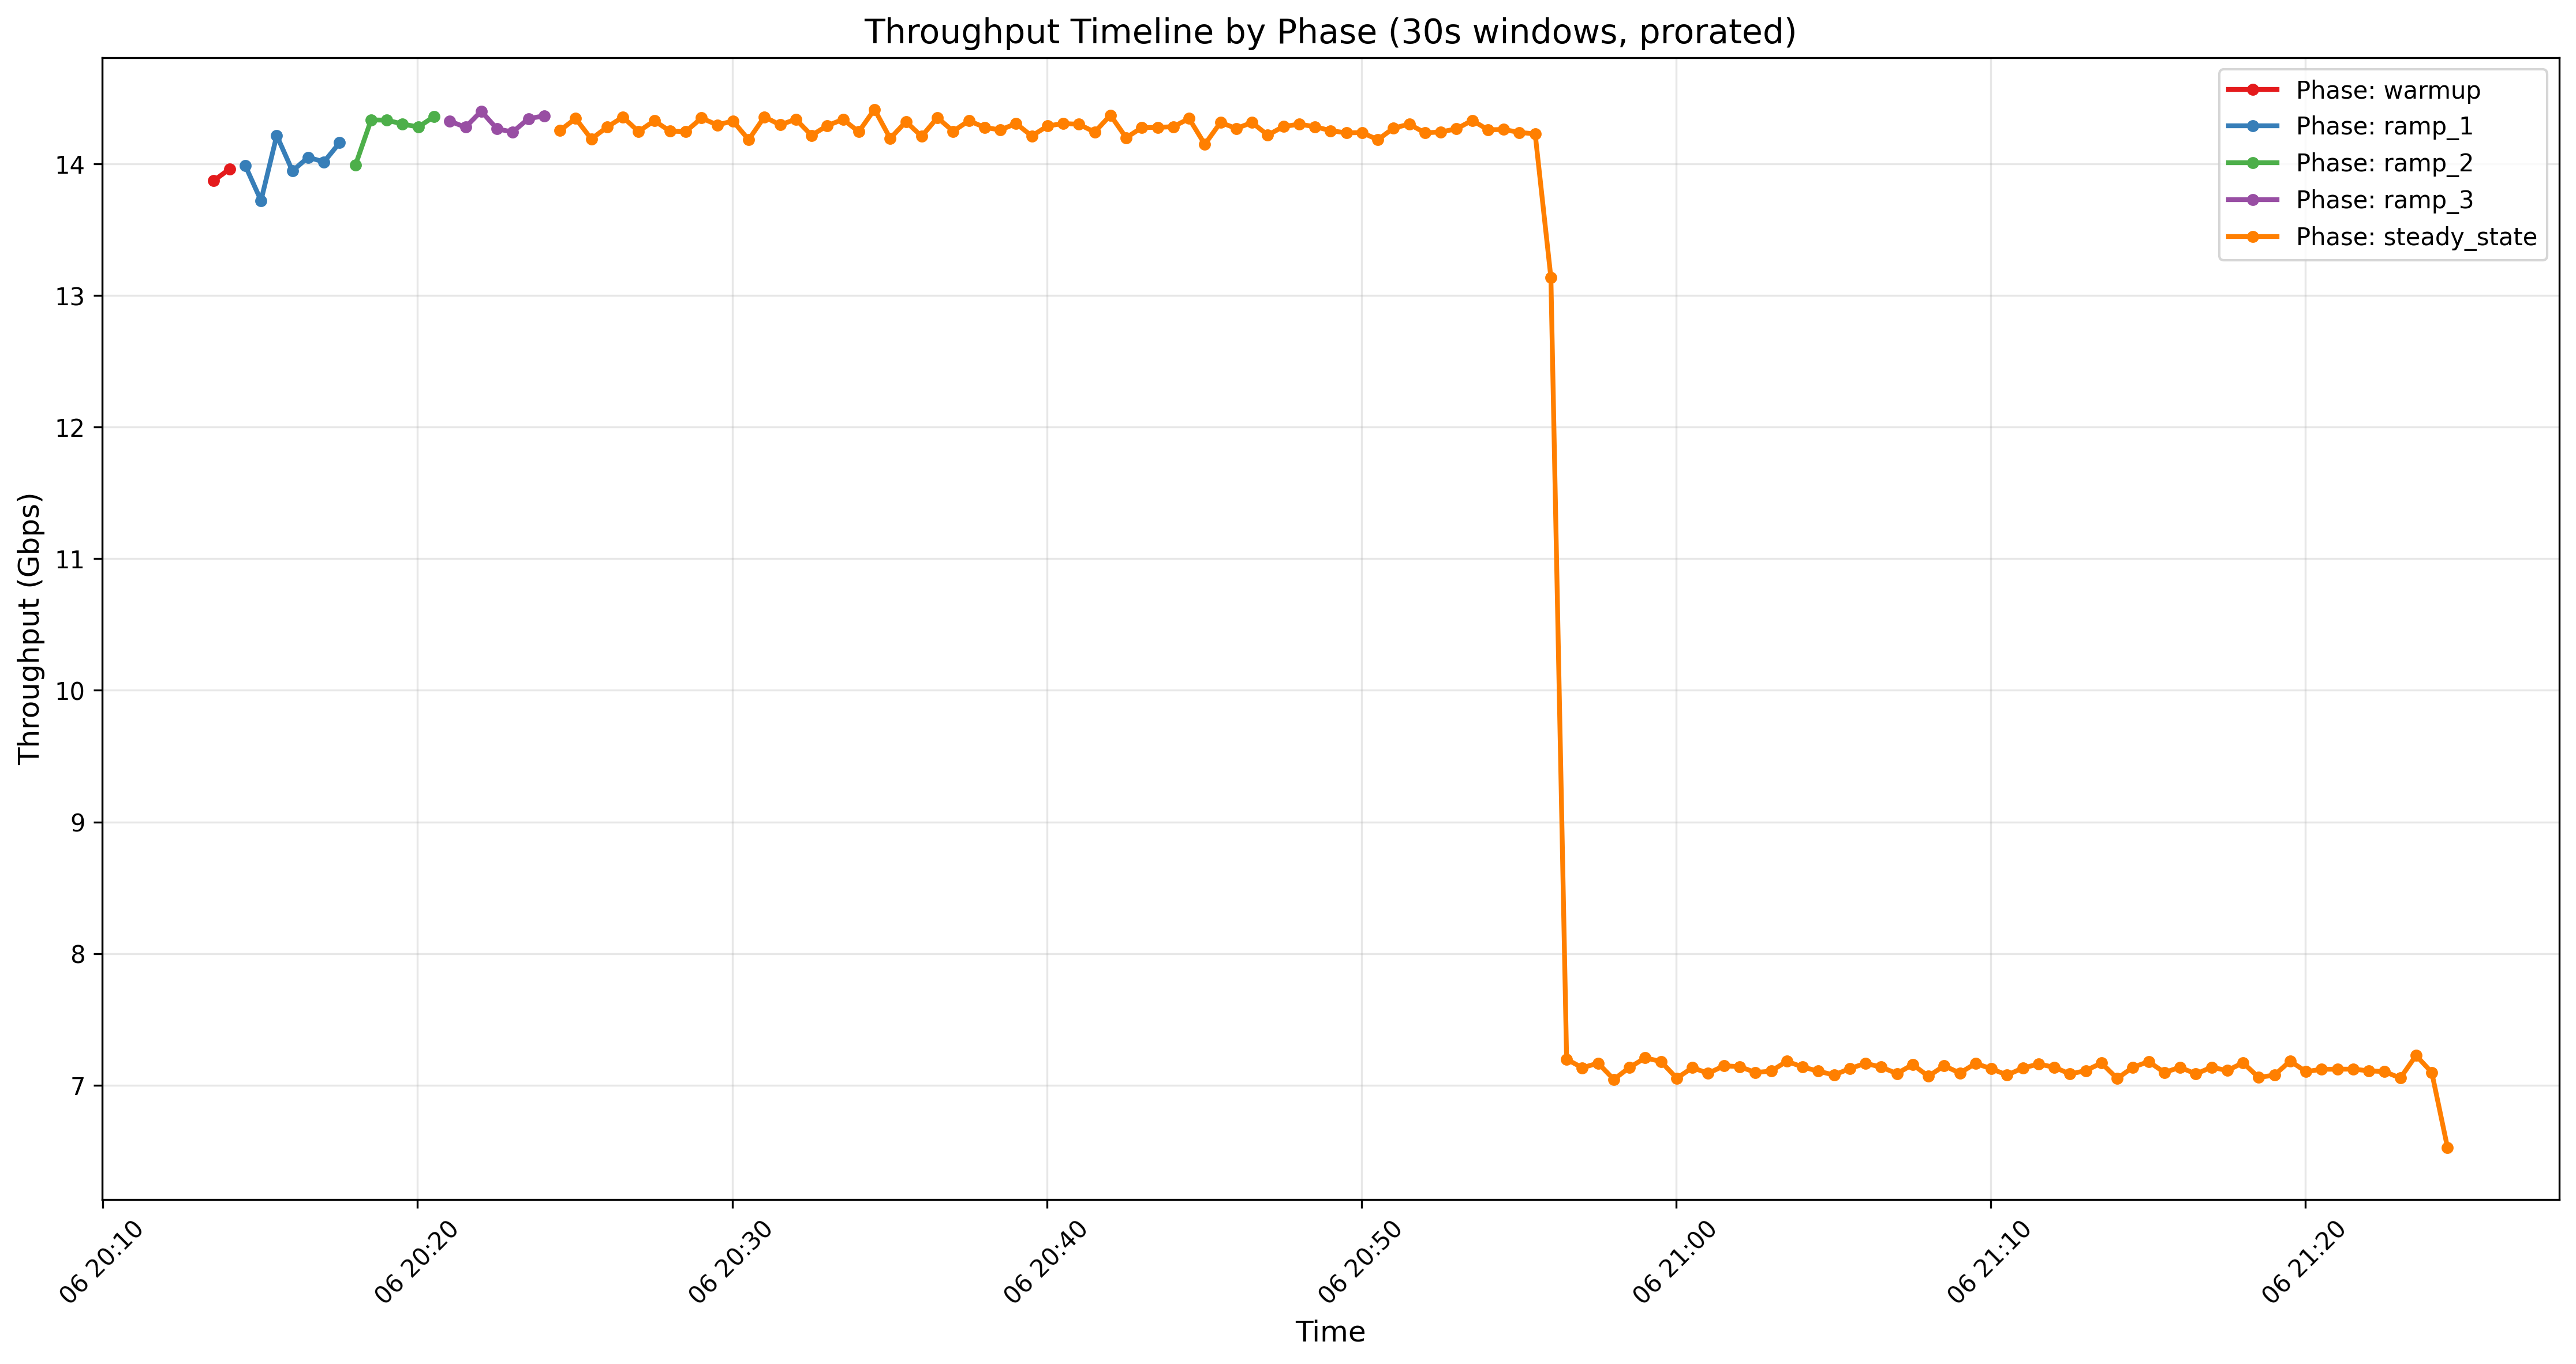
\includegraphics[width=\textwidth]{figures/r8gd-4xlarge-2-throughput_timeline.png}
\caption{Throughput timeline for r8gd.4xlarge-2 (100 MB / p=3, 1.19 hours): initial elevated period at $\approx$14.2 Gbps followed by a permanent step-down to $\approx$7.1 Gbps under sustained load. r8gd.4xlarge-3 shows an identical cliff at the same post-cliff level.}
\label{fig:r8gd-steady-state}
\end{figure}

A notable finding from r8gd.4xlarge-3 is that throughput during the initial elevated period is essentially \emph{concurrency-insensitive}: the warmup and all three ramp phases (C=96, C=192, C=288) all delivered 14.21--14.31 Gbps. Unlike the c6in instances where concurrency strongly affected throughput, the r8gd.4xlarge operates against a network bandwidth ceiling from its variable ``up to'' specification that is the binding constraint regardless of how many connections are open.

This paired comparison confirms the chunk-size effect observed on c6in.32xlarge. Despite r8gd.4xlarge-3 operating at higher steady-state concurrency (C=192 vs C=96), its P99 latency (13,674 ms) is lower than run 2's P99 (14,957 ms), and its P50 (3,853 ms) is substantially better than run 2's P50 (4,931 ms). The 50~MB configuration reduces per-request service time, consistent with lower queue depth and reduced RTT along the same lines as the c6in.32xlarge pair analysis in Section~\ref{sec:latency-analysis}. The result is consistent across instance types and reinforces that smaller request granularity reduces tail latency without sacrificing aggregate throughput.

\subsection{S3 Latency Context: Small Objects and Global Access}

The workloads in this study --- 50--100 MB objects under high concurrency --- represent one operational scenario. Third-party benchmarks provide latency context for other common object sizes and access patterns:

\begin{itemize}
    \item \textbf{Tigris (2025)~\cite{tigris-benchmark}:} For 1 KB objects at low concurrency, S3 P50 = 22 ms vs R2 P50 = 606 ms. For small objects, S3's same-region infrastructure provides a substantial latency advantage.
    \item \textbf{Kerkour (2024)~\cite{kerkour2024s3r2}:} S3 P99 = 52 ms for same-region 50 KB reads under low concurrency, confirming sub-100 ms tail latency when neither backend nor client is under load.
    \item \textbf{Cloudflare (2023)~\cite{cloudflare-r2-faster-s3}:} For 1 MB objects, 95th-percentile \emph{end-to-end response time} from North American vantage points to buckets in US-East (Ashburn), R2 P95 = 1,262 ms vs S3 P95 = 2,055 ms (38\% lower for R2). The same study reports separate P95 tables for EMEA, APAC, and cross-region access, with R2 ahead in each scenario; methodology pinned bucket placement for comparability to S3.
    \item \textbf{Skyrise (2025)~\cite{tu-berlin-skyrise}:} An aggregate serverless workload with many concurrent clients achieved S3 Standard median latency of 27 ms and P95 of 75 ms for smaller objects, with tail latencies exceeding 10 seconds under sustained multi-client load --- consistent with the queueing pattern observed here for R2.
\end{itemize}

Latency performance is therefore strongly workload-dependent. S3's same-region access is faster for small objects; R2's edge-relative routing is more competitive in several geographically distributed scenarios~\cite{cloudflare-r2-faster-s3}. For large objects, AWS documentation and the unsaturated measurements in Section~\ref{sec:latency-analysis} indicate comparable first-byte behaviour; under the high-concurrency conditions of this study, tail latency is governed primarily by queueing dynamics rather than that baseline first-byte range.

\subsection{Answering RQ2: Latency Behaviour Under High Concurrency}

R2's tail latencies grow roughly proportionally with concurrency, consistent with queueing-theory predictions. On c6in.32xlarge-2, a 3× increase (C768 $\to$ C2304) raised P99 by 3.7× (4,182 $\to$ 15,337 ms). The system degrades gracefully, maintaining 100\% post-retry success at 2,304 concurrent connections with a measured retry rate below 0.15\%.

RTT measurements suggest queueing or congestion pressure as a dominant latency factor at high loads: at saturation on the 100~MB configuration, 62\% of mean request time was spent waiting before transfer began. The 50~MB configuration, despite identical aggregate throughput, reduced RTT at peak concurrency from 5,925~ms to 251~ms, consistent with per-request granularity influencing queueing behaviour somewhere in the request path. The paired r8gd.4xlarge configurations corroborate this finding at a different scale: the 50~MB / p=6 configuration (C=192 steady) achieved P99 of 13,674~ms while the 100~MB / p=3 configuration (C=96 steady) reached P99 of 14,957~ms---a worse tail despite lower concurrency, consistent with the higher per-request service time of larger chunks.

\section{Cost-Performance Analysis}\label{sec:cost-performance}

The throughput and latency findings in the preceding sections establish R2's performance characteristics. This section translates those findings into economic terms: how much does replacing S3 with R2 save, at what scale does the migration become worthwhile, and for which workloads does the performance profile support the switch?

\subsection{Pricing Model Comparison}

S3 and R2 apply different cost structures across three dimensions: storage, egress, and API operations. Table~\ref{tab:pricing-comparison} summarises the published list prices as of writing~\cite{aws-s3-pricing,cloudflare-r2-pricing}.

\begin{table}[H]
\centering
\caption{S3 vs R2 pricing: storage, egress, and operations}
\label{tab:pricing-comparison}
\begin{tabular}{p{3.6cm}p{3.8cm}p{3.8cm}}
\hline
\textbf{Cost component} & \textbf{Amazon S3} & \textbf{Cloudflare R2} \\
\hline
Storage (first 50 TB)  & \$0.023 / GB / month & \$0.015 / GB / month \\
Egress to internet     & \$0.09 / GB          & \textbf{\$0.00 / GB} \\
GET operations         & \$0.40 / million     & \$0.36 / million \\
\hline
\end{tabular}
\end{table}

R2's zero egress fee is its primary differentiator. The storage cost difference (\$0.008/GB/month) is meaningful for large datasets but secondary for egress-heavy workloads. API operation costs are broadly comparable and rarely dominate at scale.

\subsection{Total Cost of Ownership at Scale}

Monthly costs depend on two independent variables: storage volume and egress volume. Table~\ref{tab:cost-analysis} shows four representative workload scales, with costs computed as:
\[
\text{Monthly cost} = S_{\text{GB}} \times r_{\text{storage}} + E_{\text{GB}} \times r_{\text{egress}} + \text{operations}
\]
where operations costs are negligible relative to storage and egress for large-object workloads such as those benchmarked here.

\begin{table}[H]
\centering
\caption{Monthly cost comparison and migration break-even at four production scales (list prices; operations omitted; S3 uses published tiered storage and egress rates; break-even based on one-time S3 data-out egress at tiered rates)}
\label{tab:cost-analysis}
\small
\begin{tabular}{p{1.8cm}p{1.2cm}p{1.4cm}p{1.6cm}p{1.6cm}p{1.6cm}p{1.2cm}p{1.8cm}}
\hline
\textbf{Scale} & \textbf{Storage} & \textbf{Egress/mo} & \textbf{S3/mo} & \textbf{R2/mo} & \textbf{Savings/mo} & \textbf{Savings} & \textbf{Break-even} \\
\hline
Small      & 10 TB  & 1 TB   & \$320    & \$150   & \$170    & 53\% & $\sim$5 mo  \\
Medium     & 50 TB  & 10 TB  & \$2,050  & \$750   & \$1,300  & 63\% & 3.5 mo      \\
Large      & 100 TB & 50 TB  & \$6,600  & \$1,500 & \$5,100  & 77\% & 1.6 mo      \\
Very large & 500 TB & 100 TB & \$19,020 & \$7,520 & \$11,500 & 60\% & $\sim$2.5 mo\\
\hline
\end{tabular}
\end{table}

The savings percentage is not monotonically increasing because at very large storage volumes (500 TB), the storage cost difference becomes substantial in absolute terms, narrowing the percentage advantage relative to the egress-dominant medium/large scales. The formula simplifies to:
\[
\text{Monthly savings} \approx E_{\text{TB}} \times \$90 + S_{\text{TB}} \times \$8
\]
where the \$90/TB egress coefficient comes from the full elimination of S3's \$0.09/GB outbound fee~($0.09 - 0.00 = \$0.09$/GB$~\times~1{,}000$~GB/TB), and the \$8/TB storage coefficient from the per-GB price difference~($0.023 - 0.015 = \$0.008$/GB/month$~\times~1{,}000$~GB/TB). This formula uses S3's first-tier flat rate and is accurate for egress up to 10 TB/month; at higher volumes S3's tiered pricing reduces the effective egress rate---the Large and Very Large rows in Table~\ref{tab:cost-analysis} use actual tiered rates, so the formula overpredicts savings above 10 TB/month egress. Egress savings dominate for active datasets; storage savings accumulate regardless of access frequency.

\subsection{Migration Cost and Break-Even}\label{sec:migration-break-even}

Migrating from S3 to R2 incurs a one-time egress cost (data transfer out of S3 to Cloudflare) and engineering effort. Cloudflare provides two migration paths~\cite{cloudflare-super-slurper,cloudflare-sippy}: Super Slurper for bulk migration and Sippy for incremental on-demand migration that avoids upfront egress costs by copying objects lazily as they are requested.

Break-even figures are shown directly in Table~\ref{tab:cost-analysis}. At small scale (10 TB data, \$170/month savings), the one-time S3 egress bill of approximately \$900 yields a payback of roughly 5 months. For the medium-scale workload (50 TB data, \$1,300/month savings), a one-time egress bill of approximately \$4,500 represents a 3.5-month payback. At large scale (100 TB data, \$5,100/month savings), approximately \$8,000 in egress costs (using tiered S3 rates) yields a 1.6-month payback. For very large workloads (500 TB data), tiered egress rates reduce the per-TB migration cost, giving a payback of approximately 2.5 months despite the higher absolute bill. For all four scales, break-even falls well within a year, and for egress-dominant large workloads it is typically reached within two billing cycles.

\subsection{Performance Constraints on the Cost Case}

The cost savings are only actionable if R2's performance profile is acceptable for the workload. The benchmarks in Sections~\ref{sec:throughput-analysis} and~\ref{sec:latency-analysis} provide the relevant constraints:

\begin{itemize}
    \item \textbf{Large-object bulk transfers} (50--100 MB objects, batch pipelines, backups): R2 achieved up to 114 Gbps from a single EC2 instance, within the same order of magnitude as S3's documented single-instance reference figure~\cite{aws-s3-performance}. Since the client was the bottleneck in both cases, neither system's actual backend ceiling was reached; cost savings can be pursued without observed performance penalty at single-instance scale.

    \item \textbf{Latency-tolerant high-concurrency workloads}: R2 maintained 100\% success rates at 2,304 concurrent connections with predictable, sub-linear latency growth. Tail latency is tunable via concurrency and chunk size configuration.

    \item \textbf{Small-object, latency-sensitive workloads} ($<$1 MB per request): third-party benchmarks show S3 achieving 22 ms P50 for 1 KB objects~\cite{tigris-benchmark} vs R2's 606 ms. For APIs or real-time applications, S3 is faster in same-region access and the cost savings do not compensate for the latency penalty.

    \item \textbf{Geographically distributed access}: Cloudflare's published comparison~\cite{cloudflare-r2-faster-s3} reports lower P95 end-to-end latency for R2 than for S3 for 1 MB objects across North America, EMEA, APAC, and cross-region scenarios; the headline North America/US-East figures show a 38\% P95 advantage for R2. Where user bases are spread across regions, this pattern can compound the egress cost case.
\end{itemize}

\subsection{Answering RQ3: Cost-Performance Trade-Off}

R2 offers substantial cost reductions for egress-heavy workloads: 53--77\% monthly savings depending on the egress-to-storage ratio, with break-even on migration costs typically within weeks for any workload exceeding a few terabytes per month of outbound traffic. For large-object bulk transfers --- the workload class benchmarked in this study --- the measured throughput is comparable to S3 at the client scale tested; since the client was the bottleneck in both cases, neither system's true backend ceiling was reached. For small-object or latency-sensitive workloads, S3's lower per-request latency in same-region access makes it the better choice regardless of cost.

The cost case must be evaluated against realistic achievable throughput for the specific client implementation. For high-throughput pipelines using non-Python clients, R2's performance profile may differ from what this study measured; the 114 Gbps figure reflects a client-side ceiling, not an R2-side limit. The principal migration risk is not throughput but operational: applications relying on S3-specific features (Object Lock, Intelligent-Tiering, S3 Select) require adaptation. For egress-intensive workloads with large objects --- data pipelines, media distribution, ML training data, backup archives --- R2 presents a straightforward cost reduction with throughput that is, at minimum, comparable to S3 at single-instance scale.

\section{Limitations and Threats to Validity}\label{sec:limitations}

The findings of this study are bounded by several experimental constraints that affect the generalizability of conclusions.

\textbf{Client-side bottleneck and variable bandwidth.} The Python-based client saturated CPU on all instances above 15~Gbps, making throughput figures lower bounds on what R2 can serve. For the two ``up to'' bandwidth instances (r5.xlarge and r8gd.4xlarge), the short test durations (14 and 11--13 minutes) fall within the initial elevated-bandwidth period observed on the r8gd long-run experiments (cliff at 28--37 minutes); the r5.xlarge's sustained floor was not characterised. The 32+ vCPU instances carry fixed bandwidth specifications and are not subject to this concern. The r8gd is the only instance class for which the post-cliff sustained throughput was empirically established.

\textbf{Single-object workload.} All tests targeted byte-range GET requests against a single 9 GB object. Production workloads typically span millions of objects across many prefixes. Single-object range requests may concentrate load on a limited set of storage partitions, potentially underestimating the achievable throughput in multi-object scenarios where load is distributed across the storage cluster. Storage systems may also internally optimise or cache single-object access patterns differently from realistic distributions. In a multi-object workload, one would additionally expect metadata index pressure and prefix routing overhead---both of which could affect throughput and latency relative to the figures measured here.

\textbf{Large-object focus.} Chunk sizes of 50--100 MB are representative of batch data pipelines and media processing, but not of interactive API workloads or small-object key-value access. Third-party benchmarks (Section~\ref{sec:latency-analysis}) show that R2's latency profile for objects below 1 MB differs substantially; results from this study do not generalise to those workloads.

\textbf{S3 measurements from a different framework version.} The S3 baseline data referenced in Section~\ref{sec:latency-analysis} was collected using an earlier iteration of the benchmarking framework. Differences in connection pooling and retry behaviour may affect comparability; S3 figures are used only to confirm order-of-magnitude baseline first-byte latency, not for precise numerical comparison.

\textbf{No network path instrumentation.} RTT measurements capture end-to-end delay but do not decompose it into backend processing time, TCP round-trip, and intermediate buffering. The Frankfurt vs.\ Stockholm throughput difference (Section~\ref{sec:throughput-analysis}) is attributed to network path quality differences, but without traceroute data, RTT baselines to Cloudflare PoPs, or BGP path analysis the specific cause cannot be verified. Future work should instrument the network path using tools such as \texttt{traceroute}, TCP socket metrics (\texttt{ss -ti}), or packet captures to isolate backend latency from network propagation delay.

\textbf{Opaque R2 bucket placement.} Cloudflare does not expose the physical location of R2 buckets; placement is determined automatically based on where the bucket was first written, with only coarse-grained jurisdiction hints available to the user~\cite{kerkour2024s3r2}. All experiments assumed proximity between the EC2 instances and R2's storage backend, but this cannot be verified. If the bucket was placed in a Cloudflare region geographically distant from Frankfurt or Stockholm, the measured RTT values would include inter-region latency, making the absolute RTT figures in Section~\ref{sec:latency-analysis} an overestimate of R2's intrinsic backend latency.

\textbf{Limited regional scope.} All experiments used AWS instances in two EU regions (eu-north-1 Stockholm and eu-central-1 Frankfurt) connecting to Cloudflare's R2 storage; all r8gd.4xlarge runs and the c6in.32xlarge-3 cross-region comparison used Frankfurt. Results may differ in other geographic regions where Cloudflare's network topology or R2 PoP placement differs.

\textbf{Post-retry success rates.} The 100\% success rates reported throughout reflect outcomes after up to three automatic retries per request. Transient error rates (measured at approximately 0.048\% on r8gd.4xlarge-3) are masked in aggregate metrics. Applications that cannot tolerate retries face a non-zero transient failure rate at high concurrency.
